\documentclass[letter, 10pt]{article}
\usepackage[utf8]{inputenc}
\usepackage[activeacute,spanish,es-lcroman]{babel}
\usepackage{graphicx}
\usepackage{url}
\usepackage[top=3cm,bottom=3cm,left=3.5cm,right=3.5cm,footskip=1.5cm,headheight=1.5cm,headsep=.5cm,textheight=3cm]{geometry}

\usepackage{amsfonts}
\usepackage{amsmath}
\usepackage{amssymb}

\usepackage{adjustbox}
\usepackage{changepage}
\usepackage{float}

\usepackage{enumerate}
\usepackage{enumitem}

\usepackage{cases}

\usepackage{empheq}

\usepackage{fancybox}

\usepackage{subcaption}

\usepackage{hyperref}

\usepackage{algorithm}
\usepackage{algpseudocode}

\floatname{algorithm}{Algoritmo}


\begin{document}
\title{Inteligencia Artificial \\ \begin{Large}Resolviendo el 2D Strip Packing Problem con Hill Climbing\end{Large}}
\author{Maximiliano Sepúlveda Alvear}
\date{\today}
\maketitle


\vspace{2cm}


\begin{abstract}

    El 2D Strip Packing Problem (2DSP) es un problema que busca una forma óptima de distribuir diferentes elementos dentro de un contenedor en dos dimensiones de ancho fijo y altura infinita. Este problema posee diversas aplicaciones prácticas en la vida real en procesos cercanos al corte de material. Sin embargo, no es fácil calcular la mejor solución. Diversos autores en la literatura han aportado con diferentes métodos y heurísticas para obtener soluciones a diferentes casos. En este informe se estudia el estado del arte del 2DSP: su definición, variantes más conocidas, modelo matemático, métodos y heurísticas estudiadas en la literatura. Finalmente se presenta una propuesta de implementación y solución utilizando una heurística avariciosa de Hill Climbing para resolver el problema, junto con los resultados obtenidos.

\end{abstract}




\section{Introducción}

Los problemas de empaquetamiento son un tipo de problema combinatorio que busca encajar múltiples ``paquetes'' de diferentes tamaños y formas dentro de un contenedor más grande con tal de usar el menor espacio posible. Este problema tiene diferentes variantes dependiendo de las dimensiones y restricciones como rotaciones, cortes, pesos, entre otros. Este tipo de problemas se les conoce como problemas de empaquetamiento o \textit{packing problems}. Existen diversas variantes de este problema, y en esta lectura se estudiará el empaquetamiento en tiras en dos dimensiones, o \textit{2D Strip Packing Problem} (2DSP).

Este problema posee diversas aplicaciones prácticas en la industria manufacturera, por ejemplo: en la industria textil, de corte láser, de corte de madera, entre otros, donde se busca cortar la mayor cantidad de piezas con el menor desperdicio de material posible. Por esta razón, la industria le da un gran valor e importancia al estudio de este problema, ya que les ayuda a ahorrar recursos y dinero. En aplicaciones menos frecuentes, los empaquetamientos también pueden adaptarse a la gestión de horarios, donde se busca acomodar la mayor cantidad de eventos en algún día, con el menor tiempo de espera entre eventos. Además, también se puede aplicar a la distribución de contenedores en un barco en donde el peso de estos es relevante para mantener el equilibrio. Con lo anterior, se busca la motivación en el lector para el estudio de este problema, considerando las variadas utilidades que tiene.

En esta lectura se explorará el estado actual del 2DSP, incluyendo su evolución en el tiempo, los aportes más relevantes e influyentes y diversas variantes que intentan acercarse a una aplicación más práctica de la vida real. El propósito de esta lectura consiste en dar un punto de entrada al conocimiento del problema, con tal que futuros investigadores que estén iniciando en el tema puedan tener una idea general de lo que se ha hecho hasta ahora y asi poder continuar en la búsqueda de mejores soluciones.

Sobre la estructura, se comienza con una definición informal del problema, junto a las variantes más conocidas. Luego se explora el estado del arte, un poco de historia, descubrimiento de heurísticas influyentes, comparaciones y resultados obtenidos de los autores. Después se presenta una definición formal y matemática, presentando el modelo, restricciones y la función que se desea optimizar. Luego se propone una resolución del problema basado en una heurística por niveles, donde su resolución sigue una aproximación \textit{Hill Climbing}. Se muestran los resultados de esta implementación con métricas, y comparaciones a los resultados obtenidos por otros autores. Finalmente se presentan las conclusiones del estudio realizado, discutiendo el estado actual del problema y posibles lineamientos para futuras investigaciones.




\section{Definición del Problema}

Los problemas de empaquetamiento o \textit{Bin Packing Problems} (BPP) son una familia de problemas que consisten en encajar rectángulos de diferentes tamaños dentro de un contenedor rectángulo de ancho y altura fija. El objetivo de este problema es acomodar los rectángulos de tal forma que el area total que forman estos sea la más baja posible. \cite{dowsland1991Packing} \cite{chung82Packing}. Se puede decir que los BPP son los problemas más generales de esta naturaleza, y que a partir de allí nacen las diversas variantes que existen.

Dyckhoff \cite{dyckhoff1990Typo} y Wäsher \cite{wascher2007Typo} caracterizan diferentes variantes del BPP, por dimension, restricciones, optimización, tipos de corte, entre otros. Algunos de estos pueden ser el \textit{Cutting Stock Problem}, \textit{Identical ítem Packing Problem} e incluso el \textit{Knapsack Problem}. También se abordan restricciones que acercan el problema a un entorno más realista. Algunas de estas son: si los rectángulos tienen pesos asociados, la gravedad es relevante, el contenedor es guillotinable (que se puede cortar en diferentes partes), el contenedor se puede separar en diferentes niveles, como también si los rectángulos se pueden apilar, los rectángulos pueden rotar (en 90 grados), el camino de ingreso del rectángulo o la forma de extraer los rectángulos del contenedor es relevante, entre otros.

Sin embargo, el estudio ha demostrado que es un problema fuertemente NP-Difícil, y por ende, todas sus variantes en diferentes dimensiones son igual o más difíciles de resolver. \cite{gilmore1961linear} \cite{hochbaum1985approximation} Es por esta razón que en realidad no se estudia el problema original, sino variantes con relajaciones y métodos heurísticos para resolverlas.

La variante más estudiada es el 2DSP \cite{dyckhoff1990Typo}, porque es una relajación considerable del BPP, es más sencillo de modelar, y su optimización implica multiples beneficios en aplicaciones prácticas. Este se caracteriza principalmente porque la dimension del problema es abierta: en donde el contenedor posee un ancho fijo pero una altura infinita, como si fuese un rollo de algún material, como se ve en la Figura \ref{fig:rollo}. El objetivo de este problema consiste en acomodar los diferentes rectángulos dentro del contenedor de tal forma que la altura total que utilizan sea la menor. \cite{lodi2002Survey}

\begin{figure}[h]
    \centering
    \begin{subfigure}[b]{0.45\textwidth}
        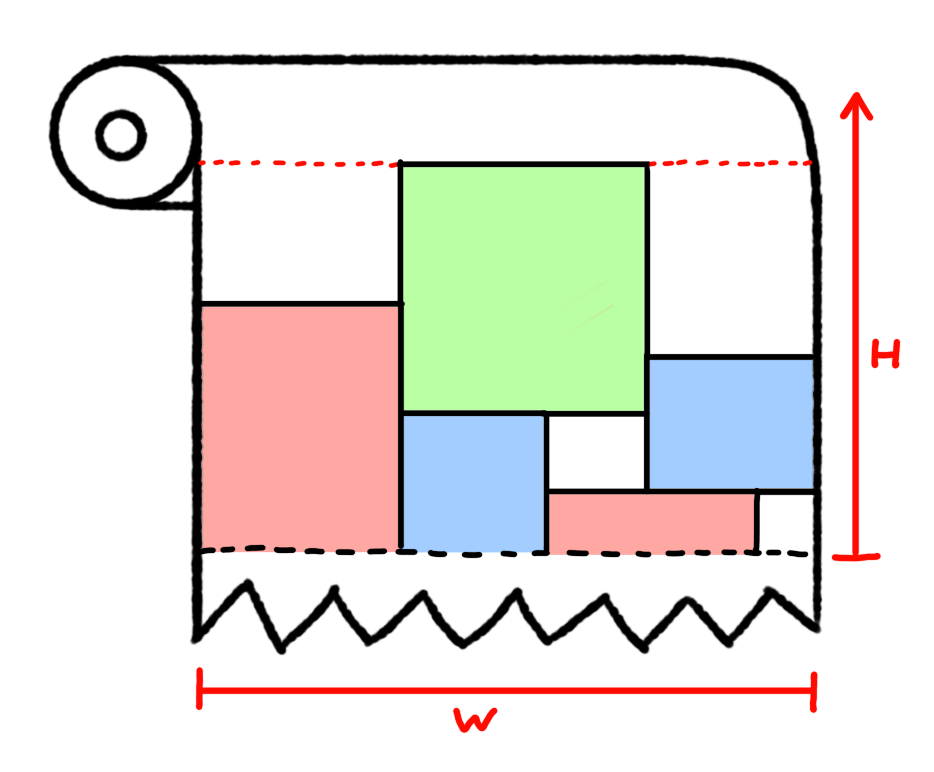
\includegraphics[width=\textwidth]{./img/rollo.png}
        \caption{Contenedor de altura infinita.}
        \label{fig:rollo}
    \end{subfigure}
    \hfill
    \begin{subfigure}[b]{0.45\textwidth}
        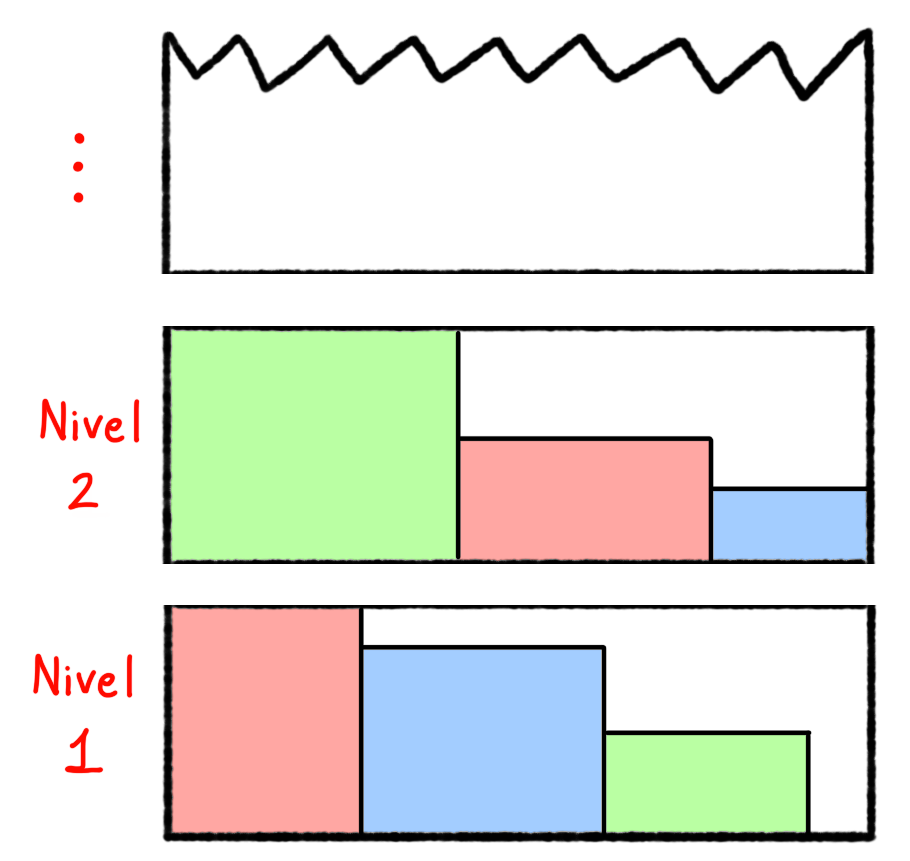
\includegraphics[width=\textwidth]{./img/niveles.png}
        \caption{Contenedor separado por niveles.}
        \label{fig:niveles}
    \end{subfigure}
    \caption{Diagramas de contenedores.}
    \label{fig:diagr}
\end{figure}

Las variables involucradas sobre las que podemos decidir dependen de la forma en como se busca resolver. Dependiendo de la heurística, pueden ser las coordenadas de los vértices inferiores izquierdos de los rectángulos, el orden de colocación de los rectángulos, el número de niveles utilizados, entre otros. Mientras que las restricciones involucradas tienen que ver generalmente con las dimensiones del contenedor, los rectángulos, y el límite de usos. En otras palabras, los rectángulos no deben salirse del contenedor, no deben superponerse, y no pueden repetirse.

El 2DSP se puede reducir al problema de empaquetamiento clásico en dos dimensiones o \textit{2D Bin Packing Problem} (2DBP), en donde los limites del contenedor son fijos y finitos.\footnote{Nótese la diferencia: 2DSP se refiere al empaquetamiento en una ``tira'', por eso la S de \textit{Strip}. Mientras que 2DBP se refiere al empaquetamiento en un ``contenedor'', por eso la B de \textit{Bin}.} La reducción consiste en dividir la tira infinita en secciones finitas a lo largo de su altura, véase la Figura \ref{fig:niveles}. \cite{lodi2004models} Este es un ejemplo de la diversas heurísticas que se han utilizado para resolver este problema.

La forma de representar el 2DSP puede afectar la complejidad del problema a causa del espacio de búsqueda. Por ejemplo, si se decide representar los rectángulos por sus coordenadas, el espacio de búsqueda es mucho mayor que si se representan por su orden de colocación. Esto se debe a que las coordenadas de los vértices pueden tomar cualquier valor dentro del contenedor, mientras que el orden de colocación solo puede tomar valores entre 1 y $n$ (siendo $n$ la cantidad de rectángulos). También si se considera el grado de rotación, que en este caso, se limitará a rotaciones en 90 grados.





\section{Estado del Arte}


Disminuir el desperdicio de material en la industria, optimizar el espacio en bodegas y distribuir anuncios en el periódico. Todos estos son ejemplos de problemas de empaquetamiento, y vienen desde hace mucho tiempo. Gilmore y Gomory \cite{gilmore1961linear} fueron los primeros en estudiar el BPP de manera matemática. Tiempo después, Hochbaum y Shamir \cite{hochbaum1985approximation} demostraron que el problema era fuertemente NP-Difícil. Dyckhoff \cite{dyckhoff1990Typo} y Wäsher \cite{wascher2007Typo} caracterizan al BPP mediante tipologías que permiten diferenciar entre variantes y condiciones.

De lo anterior, se ha estudiado diversas maneras de resolver este problema. Técnicas exactas y enumerativas como la propuesta por Martello \cite{martello2003exact} buscan de manera extensa la mejor solución posible, sin embargo, el uso de este tipo de técnicas no es muy popular en la literatura dada la dificultad de cómputo. Otras formas de soluciones exactas como la de ``branch and bound'' propuestas por Kenmochi \cite{kenmochi2009branch} también se han estudiado. Cabe destacar que se han estudiado diferentes formas de representación del problema, como las de Fekete y Schepers \cite{fekete1997more} que utilizan grafos para modelar relaciones entre los rectángulos y el contenedor.

La primera referencia al 2DSP viene de Baker en su paper ``Orthogonal PAckings in Two Dimensions'' \cite{baker1980orthogonal}, donde se estudia el caso de un contenedor de altura infinita, y en donde el objetivo es acomodar los rectángulos de tal manera que minimice la altura utilizada.

Las técnicas más populares y estudiadas son los algoritmos de aproximación, metaheurísticas y algoritmos híbridos, ya que permiten un buen equilibrio entre encontrar la mejor solución y disminuir los tiempos de cómputo. Algunos referentes son la búsqueda en dos niveles con un algoritmo greedy \cite{chen2007twolevel}, algoritmos genéticos \cite{thomas2013hybrid} \cite{hopper2001empirical}, heurísticas como ``fruit fly optimization'' \cite{babaoglu2017fruit} \footnote{\textit{Fruit Fly Optimization} consiste en comenzar con varias ``moscas'' en múltiples puntos del espacio de búsqueda. De entre todas las moscas, quien tenga la mejor solución, se define como optimo global. Luego, cada mosca irá moviéndose de manera aleatoria, y se comparan las soluciones con la solución global obtenida anteriormente.} y ``skyline'' \cite{wei2011skyline} \footnote{La heurística \textit{Skyline} consiste en ir acomodando los rectángulos considerando los bordes superiores de los rectángulos, como si fuese una silueta de una ciudad, llamada ``Skyline''. En cada iteración, esta silueta cambia, definiendo nuevos limites para ingresar rectángulos.}. En cuanto a resultados obtenidos, se puede decir que la heurística ``skyline'' ha sido el que mejores ha obtenido en diferentes pruebas \cite{wei2011skyline}. Actualmente se está prefiriendo métodos metaheurísticos para resolver el problema, como machine learning, algoritmos genéticos y búsqueda tabú.

Sobre las dificultades que hay actualmente, tiene que ver con las instancias de referencia. Hace falta un conjunto amplio y diverso, que permita evaluar y comparar el desempeño de los distintos algoritmos propuestos. Algunos autores han usado instancias generadas aleatoriamente, mientras que otros han usado instancias reales o adaptadas de otros problemas. También resulta complejo definir una metodología estándar para medir la calidad de las soluciones obtenidas por los algoritmos. Algunos autores han usado el valor absoluto de la altura de la tira como criterio, mientras que otros han usado el valor relativo respecto a una cota inferior o a una solución conocida. Por último, la diversidad y especificidad de las restricciones adicionales que pueden presentarse en las aplicaciones reales del problema afectan en la complejidad de los algoritmos que se estudian.







\section{Modelo Matemático}

De los diversos modelos matemáticos que existen en la literatura, se presenta el de Lodi, Martello y Vigo \cite{lodi2004models}. Estos consideran la resolución del problema utilizando una estrategia por niveles usando un modelo de programación lineal entero (ILP). Los autores lo denominan como \textit{2D Level Bin/Strip Packing Problem} (2LBP/2LSP).

Se posee un conjunto $J$ de $n$ rectángulos, que a partir de ahora llamaremos \textbf{ítems}. Cada ítem $j \in J = \{1,...,n\}$ tiene un ancho $w_j$ y altura $h_j$ asociada. Los contenedores poseen un ancho $W$ y una altura $H$ fija para todos.

Como restricción general, ningún ítem debe superar por completo las dimensiones del contenedor, es decir $w_j \leq W$ y $h_j \leq  H$ para todo $j \in J$.

Para este modelo, se consideran tres supuestos:

\begin{enumerate}[label=(\roman*)]
    \item En cada nivel, el ítem más a la izquierda es el más alto.
    \item En cada contenedor, el nivel más inferior es el más alto.
    \item Los ítems son ordenados y re-enumerados de manera descendiente según su altura, es decir: $h_1 \geq  h_2 \geq \cdots \geq h_n$ \footnote{El primer rectángulo en la lista tiene la mayor altura, el último, la menor.}
\end{enumerate}

Considerando esto, el orden de cada nivel es de izquierda a derecha, y de cada contenedor es de abajo hacia arriba. Ahora, si un ítem es el primero de un nivel, se dice que este \textit{inicializa} el nivel. De manera similar, si un nivel es el primero en un contenedor, se dice que este \textit{inicializa} el contenedor. Con esto, la altura de cada nivel es determinada por el ítem quien lo inicializa, es decir, el más alto. Véase la Figura \ref{fig:conts}.

\begin{figure}[h]
    \centering
    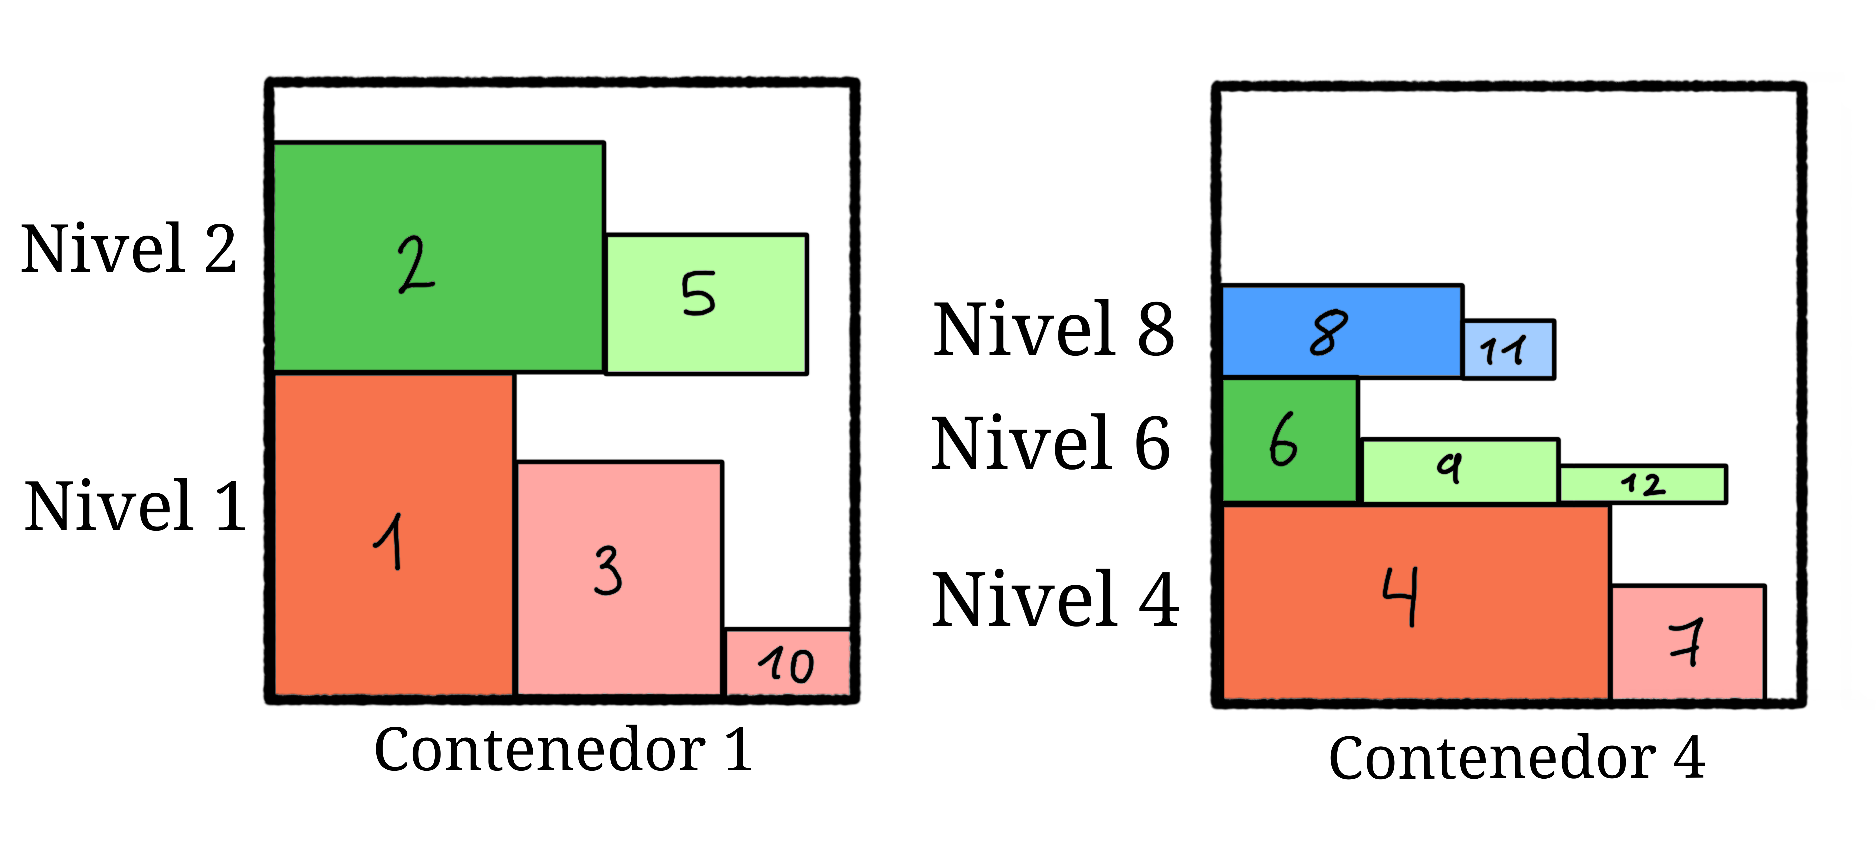
\includegraphics[width=0.8\textwidth]{./img/conts.png}
    \caption{Contenedor con niveles.}
    \label{fig:conts}
\end{figure}

Primero definimos el modelo para el 2LBP. Hay cuatro variables binarias, las primeras dos tienen relación con los ítems en los niveles, y las otras dos con los niveles en los contenedores.

\begin{equation}
    y_i = \begin{cases}
        1 & \text{si el ítem $i$ inicializa el nivel $i$} \\
        0 & \text{en caso contrario}
    \end{cases} \quad \forall i = 1,\ldots,n
\end{equation}

\begin{equation}
    x_{ij} = \begin{cases}
        1 & \text{si el ítem $j$ está en el nivel $i$} \\
        0 & \text{en caso contrario}
    \end{cases} \quad \forall i = 1,\ldots,n-1; \quad j>i
\end{equation}

\begin{equation}
    q_k = \begin{cases}
        1 & \text{si el nivel $k$ inicializa el contenedor $k$} \\
        0 & \text{en caso contrario}
    \end{cases} \quad \forall k = 1,\ldots,n
\end{equation}

\begin{equation}
    z_{ki} = \begin{cases}
        1 & \text{si el nivel $i$ está en el contenedor $k$} \\
        0 & \text{en caso contrario}
    \end{cases} \quad \forall k = 1,\ldots,n-1; \quad i>k
\end{equation}

Es útil notar que el índice $j$ corresponde a los ítems, $i$ a los niveles y $k$ a los contenedores. Sobre las condiciones de los índices: $j > i$ nace de los supuestos (i) y (iii) y $i > k$, de (ii) y (iii). El primero hace relación a que las alturas de los ítems $j$ que están en un nivel deben ser necesariamente más pequeños que el ítem que inicializa dicho nivel $i$. De manera análoga, el segundo indica que las alturas de los niveles $i$ de un contenedor deben ser necesariamente más pequeños que la altura del nivel que inicializa dicho contenedor $k$.

Con las variables a utilizar ya definidas, se presenta el modelo de optimización del 2LBP:

\begin{empheq}[box=\shadowbox*]{align}
    \text{min   } & \sum_{k=1}^{n} q_k \\
    \text{sujeto a   } & \sum_{i=1}^{j-1}{x_{ij} + y_j} = 1 & \forall j = 1,...,n \\
    & \hspace{-0.5em} \sum_{j=i+1}^{n}{w_j \cdot x_{ij}} \leq (W - w_i) \cdot y_i & \forall i = 1,...,n-1 \\
    & \sum_{k=1}^{i-1}{z_{ki} + q_i} = y_i & \forall i = 1,...,n \\
    & \hspace{-0.5em} \sum_{i=k+1}^{n}{h_i \cdot z_{ki}} \leq (H - h_k) \cdot q_k & \forall k = 1,...,n-1 \\
    & y_i \in \{0,1\} & \forall i = 1,...,n \\
    & x_{ij} \in \{0,1\} & \forall i = 1,...,n-1; \quad j>i \\
    & q_k \in \{0,1\} & \forall k = 1,...,n \\
    & z_{ki} \in \{0,1\} & \forall k = 1,...,n-1; \quad i>k
\end{empheq}

Las restricciones (10)-(13) denotan la naturaleza de las variables.

La restricción (6) impone que cada ítem $j$ debe estar empaquetado una única vez. Esto sea inicializando el nivel con dicho ítem, o que el ítem ya esté en un nivel inicializado por otro más grande (recordar que $j > i$, es decir, el ítem $j$ es más pequeño que el ítem $i$).

De manera análoga, la restricción (8) impone que cada nivel $i$ debe estar en un único contenedor. Esto sea que el nivel inicialice el contenedor, o que el nivel ya se encuentre en un contenedor inicializado por otro más grande (recordar que $i > k$, es decir, el nivel $i$ es más pequeño que el nivel $k$).

La restricción (7) impone límites de ancho para cada nivel. Nótese que dado un nivel $i$, las comprobaciones comienzan por el ítem $i+1$, ya que el ítem $i$ es quien inicializa el nivel. Se debe comprobar si el resto de ítems $j$ de dicho nivel (de ahí la utilidad de $x_{ij}$ como variable de activación) no supera el ancho restante del contenedor ($W-w_i$).

De manera análoga, la restricción (9) impone limites de altura para cada contenedor. Nótese que dado un contenedor $k$, las comprobaciones comienzan por el nivel $k+1$, ya que el nivel $k$ es quien inicializa el contenedor. Se debe comprobar si el resto de niveles $i$ de dicho contenedor (de ahi la utilidad de $z_{ki}$ como variable de activación) no supera la altura restante del contenedor ($H-h_k$).

Finalmente, el problema de utilizar el menor espacio en los contenedores se reduce a usar la menor cantidad de contenedores. Esta es la función objetivo (5), quien busca minimizar la cantidad de contenedores usados.

Del modelo anterior, se puede derivar el modelo para el 2LSP simplemente eliminando las restricciones para la altura de los contenedores, es decir (8) y (9). El modelo de optimización para el 2LSP es el siguiente:

\begin{empheq}[box=\shadowbox*]{align}
    \text{min   } & \sum_{i=1}^{n} h_i \cdot y_i \\
    \text{sujeto a   } & \sum_{i=1}^{j-1}{x_{ij} + y_j} = 1 & \forall j = 1,...,n \\
    & \hspace{-0.5em} \sum_{j=i+1}^{n}{w_j \cdot x_{ij}} \leq (W - w_i) \cdot y_i & \forall i = 1,...,n-1 \\
    & y_i \in \{0,1\} & \forall i = 1,...,n \\
    & x_{ij} \in \{0,1\} & \forall i = 1,...,n-1; \quad j>i
\end{empheq}

Con este cambio ya no se usa la cantidad de contenedores como medida de optimización. La función objetivo (14) se redefine: ahora se busca minimizar la suma de las alturas de los niveles inicializados.

Hasta ahora no se han considerado rotaciones. Para implementar rotaciones, Lodi propone que: para cada ítem $j = 1,...,n$ se tenga un ítem alternativo $n+j$ donde $w_{n+j} = h_j$ y $h_{n+j} = w_j$. \footnote{El ítem alternativo $n+j$ es el mismo ítem $j$ pero rotado en 90 grados (esto se logra simplemente intercambiando su ancho con su altura). En otras palabras, cada rectángulo tiene un duplicado de sí mismo, pero rotado.} Esto último provoca que la cantidad de ítems aumente de $n$ a $2n$, en otras palabras: $j = 1,...,2n$. Luego, todos los ítems son reordenados de manera descendiente por su altura. \cite{lodi2004models}

Sea $\alpha_j$ el índice de la version rotada del ítem $j$, podemos limitar a que exactamente una de las dos versiones de cada ítem sea usada en la solución. Esto se logra reemplazando la restricción (15) por:

\begin{equation}
    \sum_{i=1}^{j-1}{x_{ij} + y_j} + \sum_{i=1}^{\alpha_j-1}{x_{i\alpha_j} + y_{\alpha_j}} = 1 \quad \forall j = 1,...,2n; \quad j < \alpha_j
\end{equation}

Además de reemplazar $n$ por $2n$ en todas las restricciones. Finalmente, el modelo para el 2LSP con rotaciones de 90 grados es el siguiente:

\begin{empheq}[box=\shadowbox*]{align}
    \text{min   } & \sum_{i=1}^{2n} h_i \cdot y_i \\
    \text{sujeto a   } & \sum_{i=1}^{j-1}{x_{ij} + y_j} + \sum_{i=1}^{\alpha_j-1}{x_{i\alpha_j} + y_{\alpha_j}} = 1 & \forall j = 1,...,2n; \quad j < \alpha_j \\
    & \hspace{-0.5em} \sum_{j=i+1}^{2n}{w_j \cdot x_{ij}} \leq (W - w_i) \cdot y_i & \forall i = 1,...,2n-1 \\
    & y_i \in \{0,1\} & \forall i = 1,...,2n \\
    & x_{ij} \in \{0,1\} & \forall i = 1,...,2n-1; \quad j>i
\end{empheq}


\section{Representación}

\begin{figure}[t]
    \centering
    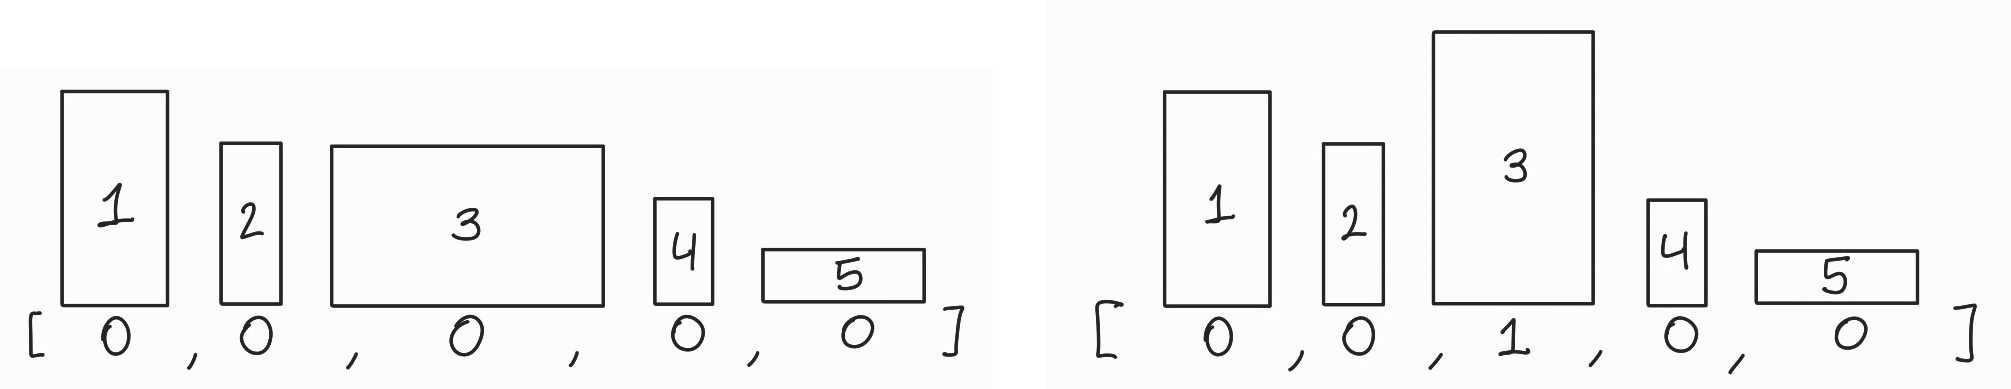
\includegraphics[width=\textwidth]{./img/rotaciones.jpg}
    \caption{Representación de rotaciones.}
    \label{fig:rot}
\end{figure}

El modelo propuesto consiste en una técnica de colocación por niveles en donde los rectángulos son ordenados por altura antes de introducirse en el contenedor. Gracias a esto, se puede prescindir de representar el orden en la solución, ya que este es determinado por la altura de los rectángulos. Sin embargo, queda pendiente la forma de representar las rotaciones de los rectángulos.

La representación de la solución que se propone es: una lista binaria de tamaño $n$ (cantidad de rectángulos), donde el índice $i$ representa al rectángulo $j$ antes de ordenar por altura.

El valor de cada elemento de la lista se lee de la siguiente manera:

\begin{equation}
    x_i = \begin{cases}
        0 & \text{si el rectángulo $i$ no está rotado}        \\
        1 & \text{si el rectángulo $i$ está rotado 90 grados}
    \end{cases} \quad \forall i = 1,...,n
\end{equation}

Esta representación permite disminuir el espacio de búsqueda, ya que se evita considerar el orden de colocación de los rectángulos, y también se evita el uso de coordenadas.

Por ejemplo: dada una lista de rectángulos $J$, la solución $[0,0,0,0,0]$ significa que ningún bloque esta rotado. En cambio la solución $[0,0,1,0,0]$ significa que el tercer bloque esta rotado, y los demás no. Véase la Figura \ref{fig:rot}.

Con esto, los vecinos de una solución se definen como todas las soluciones que se pueden obtener al cambiar el valor de un elemento de la lista. Por ejemplo: si se tiene la solución $[0,0,0,0,0]$, los vecinos son: $[1,0,0,0,0]$, $[0,1,0,0,0]$, $[0,0,1,0,0]$, $[0,0,0,1,0]$ y $[0,0,0,0,1]$.





\section{Descripción del algoritmo}

El algoritmo que se utiliza para encontrar la solución al problema es una heurística avariciosa de \textit{Hill Climbing First Improvement}. La idea es comenzar con una solución inicial, y luego ir modificando la solución de manera iterativa, hasta que no se pueda mejorar más. En cada iteración, se evalúan todos los vecinos de la solución actual, y se escoge el primero que mejore la solución. Este proceso se repite hasta que no se pueda mejorar más la solución.

La implementación del algoritmo consiste en 3 partes: el algoritmo de colocación, la prueba de instancias y el algoritmo de Hill Climbing.

Primero, el algoritmo de colocación: se recibe una lista de rectángulos $J$ y, para cada bloque, se verifica si cabe en el nivel actual. Si no cabe, se prueba el siguiente bloque en el mismo nivel. Si ningún bloque cabe en el nivel actual, se crea un nuevo nivel y el algoritmo se repite. Si el bloque cabe en el nivel actual, se agrega al contenedor y se marca como usado. El algoritmo termina cuando todos los rectángulos han sido colocados. Finalmente se retorna el área desperdiciada. Véase el Algoritmo \ref{alg:colocacion}.

Segundo, la prueba de instancias: se recibe una lista de rectángulos $J$ y una lista binaria $S$ (solución específica). Primero se ordenan los rectángulos de la lista $J$, después se rotan los rectángulos correspondientes según $S$, y luego se llama al algoritmo de colocación. Véase el Algoritmo \ref{alg:ordrot}.

Tercero, el algoritmo de Hill Climbing: se recibe una lista de rectángulos $J$ y una lista binaria $S$ (solución inicial). Primero se llama a la prueba de instancias, y se obtiene el área desperdiciada $A$. Luego se obtienen todos los vecinos de la solución $S$, y se evalúa el área desperdiciada de cada uno. Si el área desperdiciada de algún vecino es menor que $A$, se actualiza $A$ y se actualiza la solución $S$. Este proceso se repite hasta que no se pueda mejorar más la solución, lo que significa que HC se estanca en un mínimo local. Véase el Algoritmo \ref{alg:hcam}.






\section{Experimentos}

Se probó el algoritmo con diferentes cantidades de rectángulos, de tamaños variados y diferentes valores del ancho máximo del contenedor. El objetivo del experimento es observar el comportamiento del algoritmo en diferentes instancias, y comparar los resultados obtenidos con diferentes técnicas de prueba de instancias. La ejecución del algoritmo se realizó en un computador con procesador Intel Core i3-1115G4 de 3.00GHz. El algoritmo se implementó en C++ bajo un entorno Linux.

La técnica usada toma en cuenta el orden en que se colocar los rectángulos, por lo tanto, el resultado de una misma instancia siempre es el mismo. Esto es a causa de que el algoritmo de \textit{Hill Climbing} es determinista. HC termina cuando se estanca en un mínimo local o supera la cantidad de iteraciones máximas.

Sin embargo, considerando las rotaciones y el orden de los rectángulos, hay dos maneras de realizar la prueba de instancias: primero se ordenan los rectángulos y luego se rotan los correspondientes (denotado OrdRot, véase el Algoritmo \ref{alg:ordrot}), o primero se rotan los rectángulos y luego se ordenan (denotado RotOrd, véase el Algoritmo \ref{alg:rotord}). Esto puede afectar el resultado final, ya que por ejemplo: al rotar un bloque, este puede quedar más alto que otro bloque que antes era más alto.

Las instancias de prueba utilizadas consisten en grupos de 2-5 rectángulos, 6-10 rectángulos, 11-15 rectángulos y 16-20 rectángulos. Cada grupo tiene 30 instancias, para un total de 120 instancias. Las instancias poseen dimensiones variadas entre los rectángulos para verificar el comportamiento en extremos.







\section{Resultados}

\begin{figure}[b]
    \centering
    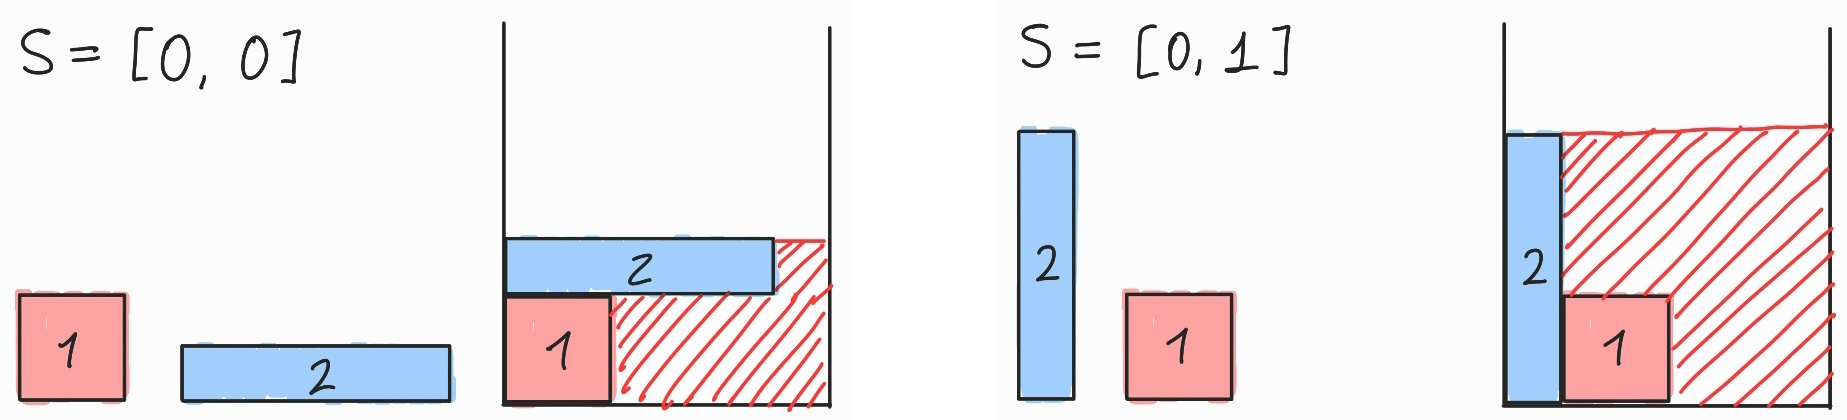
\includegraphics[width=\textwidth]{./img/diffs.jpg}
    \caption{Rectángulos variados.}
    \label{fig:diffs}
\end{figure}

Los resultados obtenidos se muestran en los siguientes gráficos, para instancias de 2-5, 6-10, 11-15 y 16-20 rectángulos. En cada gráfico se muestran los resultados para los algoritmos OrdRot y RotOrd. Véase el Anexo \ref{sec:graphs}.

Se puede notar que en la mayoría de instancias, el algoritmo RotOrd es capaz de obtener resultados mejores que OrdRot, por ejemplo: la instancia 8 y 28 de 2-5 (véase Figura \ref{fig:2-5}), la instancia 2, 7, 8 y 9 de 11-15 (véase Figura \ref{fig:11-15}), y en la instancia 8, 14 y 30 de 16-20 (véase Figura \ref{fig:16-20}).

Sin embargo, hay casos en donde RotOrd obtiene resultados peores que OrdRot, por ejemplo: la instancia 24 de 2-5 (véase Figura \ref{fig:2-5}), la instancia 28 de 6-10 (véase Figura \ref{fig:6-10}), la instancia 28 de 11-15 (véase Figura \ref{fig:11-15}), y la instancia 21 de 16-20 (véase Figura \ref{fig:16-20}).

Las instancias mencionadas anteriormente provocan una diferencia considerable entre los resultados obtenidos con OrdRot o RotOrd. Estas instancias poseen rectángulos con dimensiones muy variadas, lo que provoca que, al rotarlos, se generen rectángulos muy altos y delgados, o muy anchos y bajos. Provocando finalmente que el nivel inicializado tenga una altura muy grande, desperdiciando mucho espacio en el contenedor, o un alto muy bajo, obligando a crear un nuevo nivel. Véase la Figura \ref{fig:diffs}.

De manera análoga, las instancias que no presentan una diferencia considerable entre OrdRot y RotOrd son aquellas que poseen rectángulos con dimensiones similares. Ya que al rotar los rectángulos, estos no cambian mucho su altura, y por lo tanto, no afectan mucho el resultado final.

Sobre el tiempo de ejecución, se puede decir que ambos algoritmos son similares en su funcionamiento. Esto tiene sentido pues ambos ejecutan un algoritmo de ordenamiento antes de colocar los rectángulos.








\section{Conclusiones}

En esta lectura se introdujo el problema del empaquetamiento en dos dimensiones y hemos presentado un modelo que permite obtener una solución usando una estrategia por niveles. Sin embargo, esta última no garantiza que la solución sea óptima, dada la naturaleza difícil del problema.

Se presentó el estado del arte del 2DSP, incluyendo sus orígenes y la tendencia de los métodos utilizados para su resolución. Además de diferentes métodos estudiados en la literatura que están enfocados a diferentes objetivos de resolución.

Las técnicas exactas y exhaustivas buscan garantizar la solución óptima, sin embargo los tiempos de cómputo tienden a ser muy extensos. En cambio, técnicas heurísticas y de aproximación poseen un buen equilibrio entre tiempo de computo y la calidad de la solución. Otras técnicas se inspiran en conceptos de la física, como lo es el caso en donde los rectángulos tienen pesos asociados. Otro caso es en donde la inserción/retirada de los elementos del contenedor es relevante.

La tendencia actual en el estudio del problema sugiere que se está experimentando con metaheurísticas como algoritmos genéticos, redes neuronales, machine learning y búsqueda tabú.

Para el modelo presentado, se utiliza una técnica bastante popular en la literatura, que es el de \textit{level packing}. Esta técnica ayuda a reducir el problema del 2DSP a un problema más ``manejable'', en donde el contenedor se divide en tiras. De esta manera, las restricciones se limitan al nivel de manera local.

Se presentó una implementación de esta técnica utilizando una heurística de \textit{Hill Climbing First Improvement}. Esta heurística permite encontrar una solución de manera rápida, sin embargo, no garantiza que la solución sea óptima. Esto se debe a que HC se puede estancar en un mínimo local, y no explorar el espacio de búsqueda de manera completa.

La técnica por niveles propone ordenar los rectángulos por su altura antes de introducirlas al contenedor. Para permitir las rotaciones en la simulación, se propuso una representación de lista binaria que indica qué rectángulos son rotados.

Hay dos formas de aproximar la solución: primero ordenar los rectángulos y luego rotarlos, o primero rotar los rectángulos y luego ordenarlos. Los resultados muestran que hay una fuerte relación entre la varianza de las dimensiones de los rectángulos con los resultados de ambos métodos.

Para la industria, no es relevante encontrar la solución óptima. Sin embargo, estos modelos siguen siendo teóricos en su esencia, y no necesariamente pueden aplicar a lo que se necesita en la vida real. Por ejemplo, en el corte de metal es necesario otorgar una distancia mínima entre elementos, ya que durante el proceso, el metal se derrite cerca de los bordes, causando deformaciones. En estos casos, los modelos no presentan dichas restricciones. Aquí hay un área de oportunidad para futuras investigaciones.


\bibliographystyle{plain}
\bibliography{refs}

\appendix
\newpage
\section*{Anexo}
\section{Algoritmos} \label{sec:algs}
\begin{algorithm}[H]
    \caption{Colocación de rectángulos}
    \label{alg:colocacion}
    \begin{algorithmic}[1]
        \State $J$ \Comment{Lista de bloques}
        \State $maxW$ \Comment{Ancho máximo del contenedor}
        \Procedure{colocarBloques}{$J, maxW$}
        \State $totH \gets 0$ \Comment{Altura total usada}
        \State $totA \gets 0$ \Comment{Area total usada}
        \While{$\text{no se han colocado todos los bloques}$}
        \State $levelW \gets 0$ \Comment{Ancho usado del nivel actual}
        \State $levelH \gets 0$ \Comment{Altura usada del nivel actual}
        \For{$j \in J$}
        \If{$j \text{ no ha sido usado}$}
        \If{$j \text{ cabe en el nivel actual}$}
        \State $levelW \gets levelW + \text{Ancho}(j)$
        \State $levelH \gets \text{max}(levelH, \text{Alto}(j))$
        \State $totA \gets totA + \text{Area}(j)$
        \State $\text{marcar } j \text{ como usado}$
        \EndIf
        \EndIf
        \EndFor
        \State $totH \gets totH + levelH$ \Comment{Se agrega el nivel al contenedor}
        \EndWhile
        \State \textbf{return} $maxW \times totH - totA$ \Comment{Se retorna area desperdiciada}
        \EndProcedure
    \end{algorithmic}
\end{algorithm}



\begin{algorithm}[H]
    \caption{Prueba de Instancia: OrdRot}
    \label{alg:ordrot}
    \begin{algorithmic}[1]
        \State $J$ \Comment{Lista de bloques}
        \State $S$ \Comment{Lista bianria de rotaciones}
        \State $maxW$ \Comment{Ancho máximo del contenedor}
        \Procedure{ordRot}{$J, S, maxW$}
        \State $\text{OrdenarPorAltura}(J)$
        \For{$i \in S$}
        \If{$i = 1$}
        \State $\text{rotar bloque } i$ \Comment{Rotar bloque con la ID correspondiente}
        \EndIf
        \EndFor
        \State $result \gets \text{colocarBloques}(J, maxW)$
        \State \textbf{return} $result$
        \EndProcedure
    \end{algorithmic}
\end{algorithm}


\begin{algorithm}[H]
    \caption{Prueba de Instancia: RotOrd}
    \label{alg:rotord}
    \begin{algorithmic}[1]
        \State $J$ \Comment{Lista de bloques}
        \State $S$ \Comment{Lista bianria de rotaciones}
        \State $maxW$ \Comment{Ancho máximo del contenedor}
        \Procedure{rotOrd}{$J, S, maxW$}
        \For{$i \in S$}
        \If{$i = 1$}
        \State $\text{rotar bloque } i$ \Comment{Rotar bloque con la ID correspondiente}
        \EndIf
        \EndFor
        \State $\text{OrdenarPorAltura}(J)$
        \State $result \gets \text{colocarBloques}(J, maxW)$
        \State \textbf{return} $result$
        \EndProcedure
    \end{algorithmic}
\end{algorithm}

\begin{algorithm}[H]
    \caption{Hill Climbing Alguna Mejora}
    \label{alg:hcam}
    \begin{algorithmic}[1]
        \State $J$ \Comment{Lista de bloques}
        \State $S$ \Comment{Lista bianria de rotaciones}
        \State $maxW$ \Comment{Ancho máximo del contenedor}
        \Procedure{hillClimbing}{$J, S, maxW$}
        \State $bestA \gets \infty$ \Comment{Area desperdiciada de la mejor solución}
        \State $bestS \gets S$ \Comment{Mejor solución}
        \Repeat
        \State $mejora \gets \text{False}$
        \State $vecinos \gets \text{vecindario de } S$
        \For{$V \in vecinos$} \Comment{Se evalúan todos los vecinos}
        \State $A \gets \text{ordRot}(J, V, maxW)$
        \If{$A < bestA$}
        \State $bestA \gets A$
        \State $bestS \gets V$
        \State $S \gets V$ \Comment{Se mantiene esta solución para la siguiente iteración}
        \State $mejora \gets \text{True}$
        \State \textbf{break} \Comment{Se sale del ciclo for si se encuentra una mejora}
        \EndIf
        \EndFor
        \Until{$\text{no se encontró una mejora}$}
        \State \textbf{return} $bestA, bestS$
        \EndProcedure
    \end{algorithmic}
\end{algorithm}



\section{Gráficos} \label{sec:graphs}

\begin{figure}[H]
    \begin{adjustwidth}{-\marginparwidth}{-\marginparwidth}
        \centering
        \begin{minipage}{.5\linewidth}
            \centering
            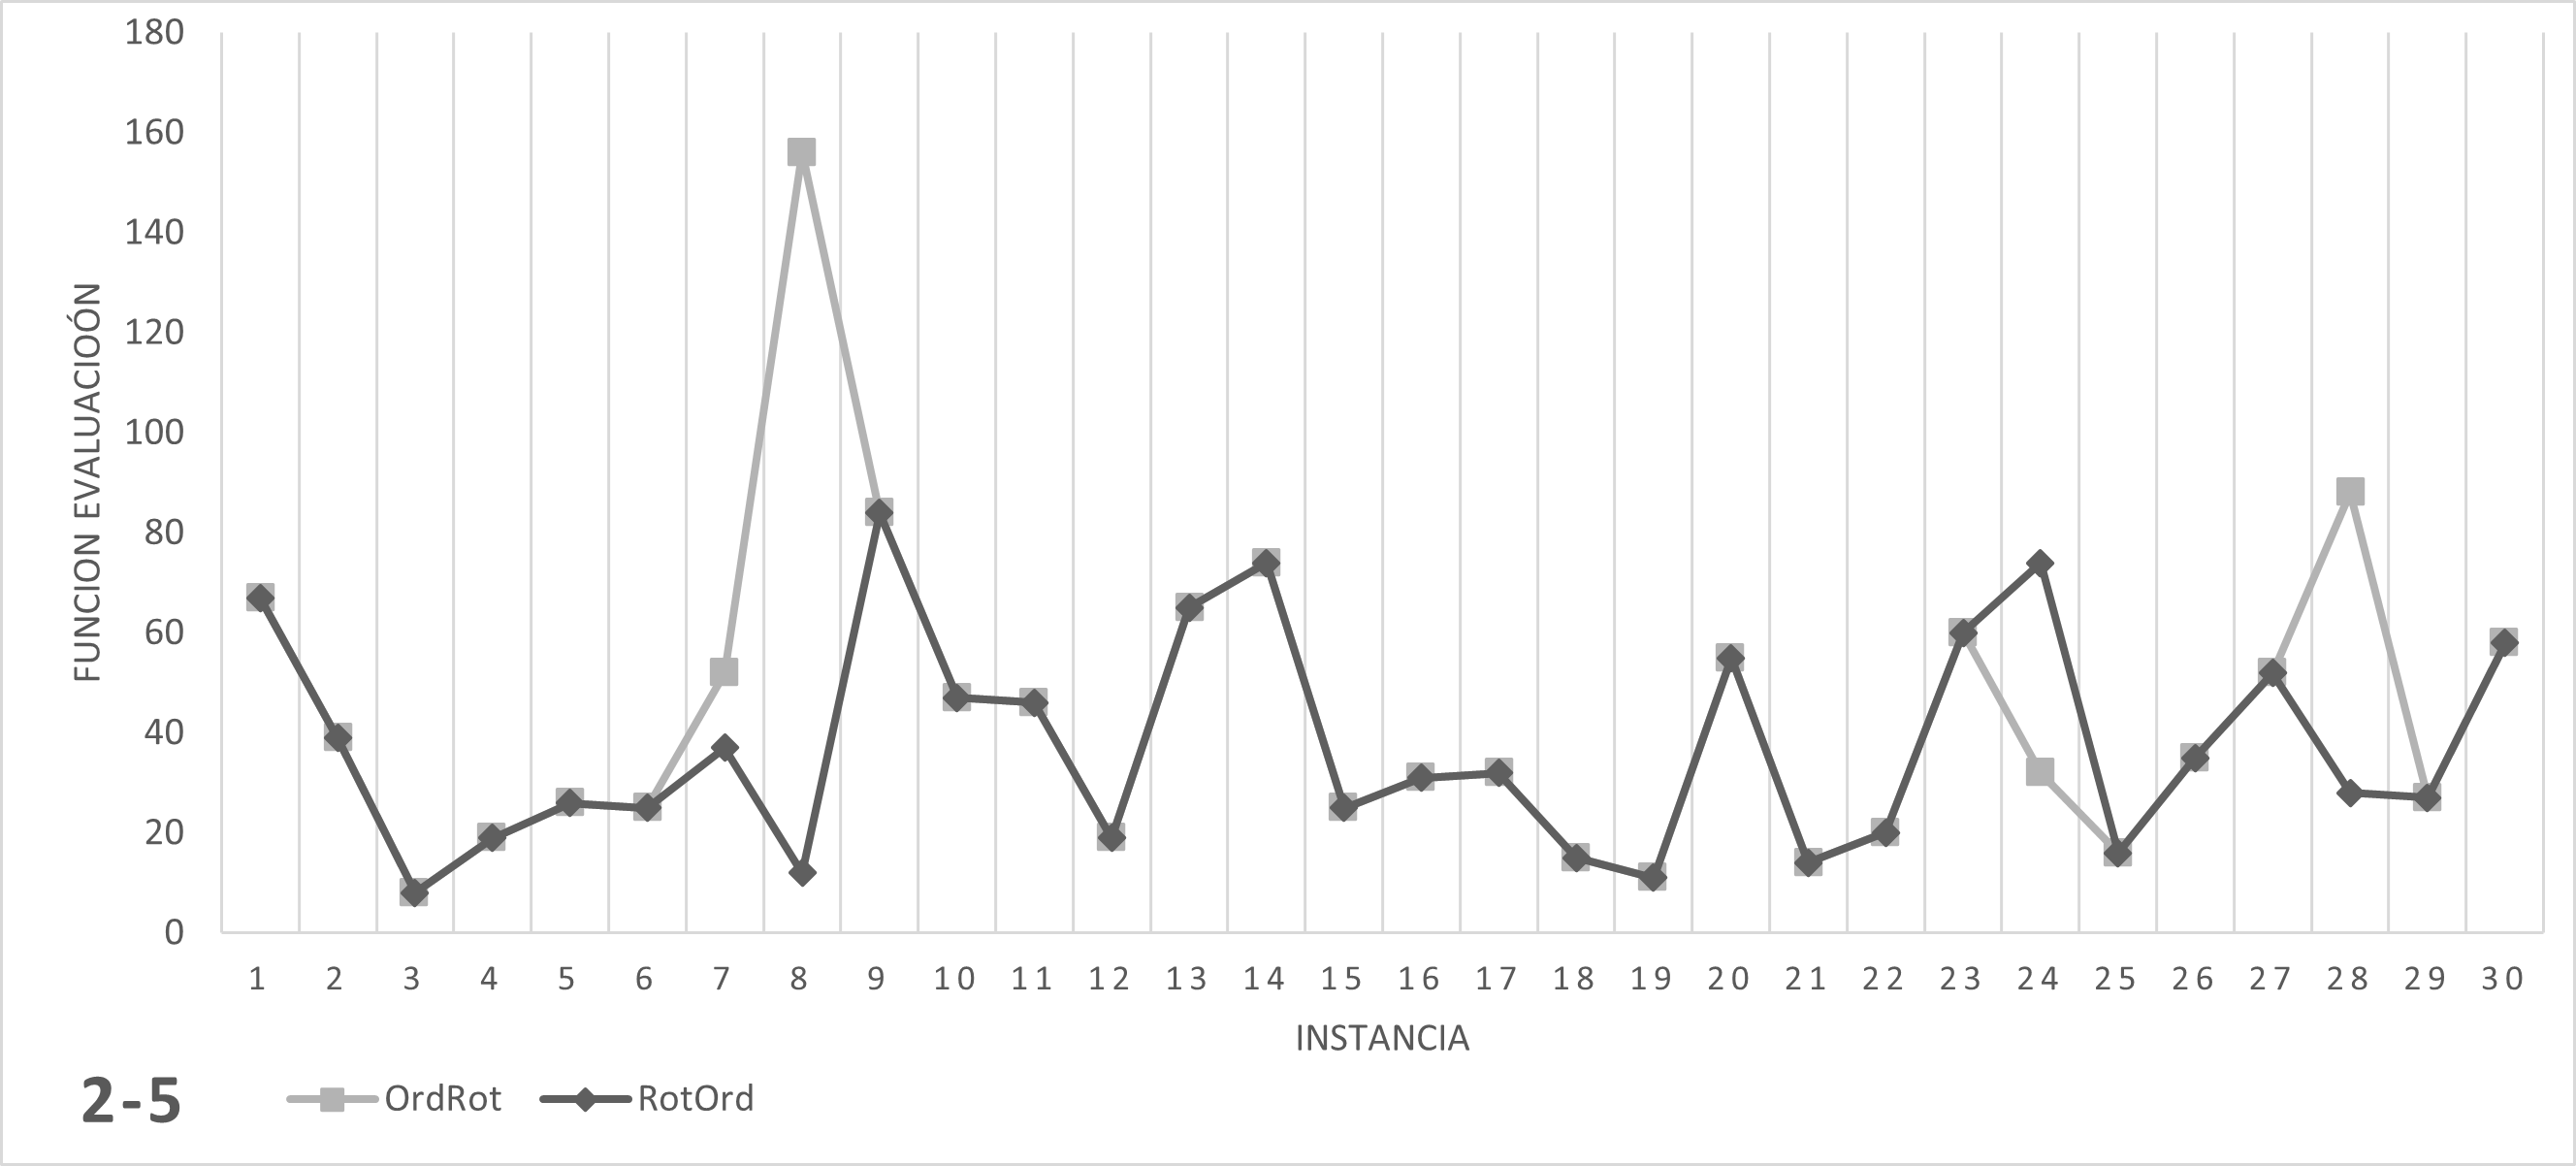
\includegraphics[width=\linewidth]{./img/2-5.png}
            \caption*{Función de evaluación.}
            \label{fig:2-5_g}
        \end{minipage}%
        \begin{minipage}{.5\linewidth}
            \centering
            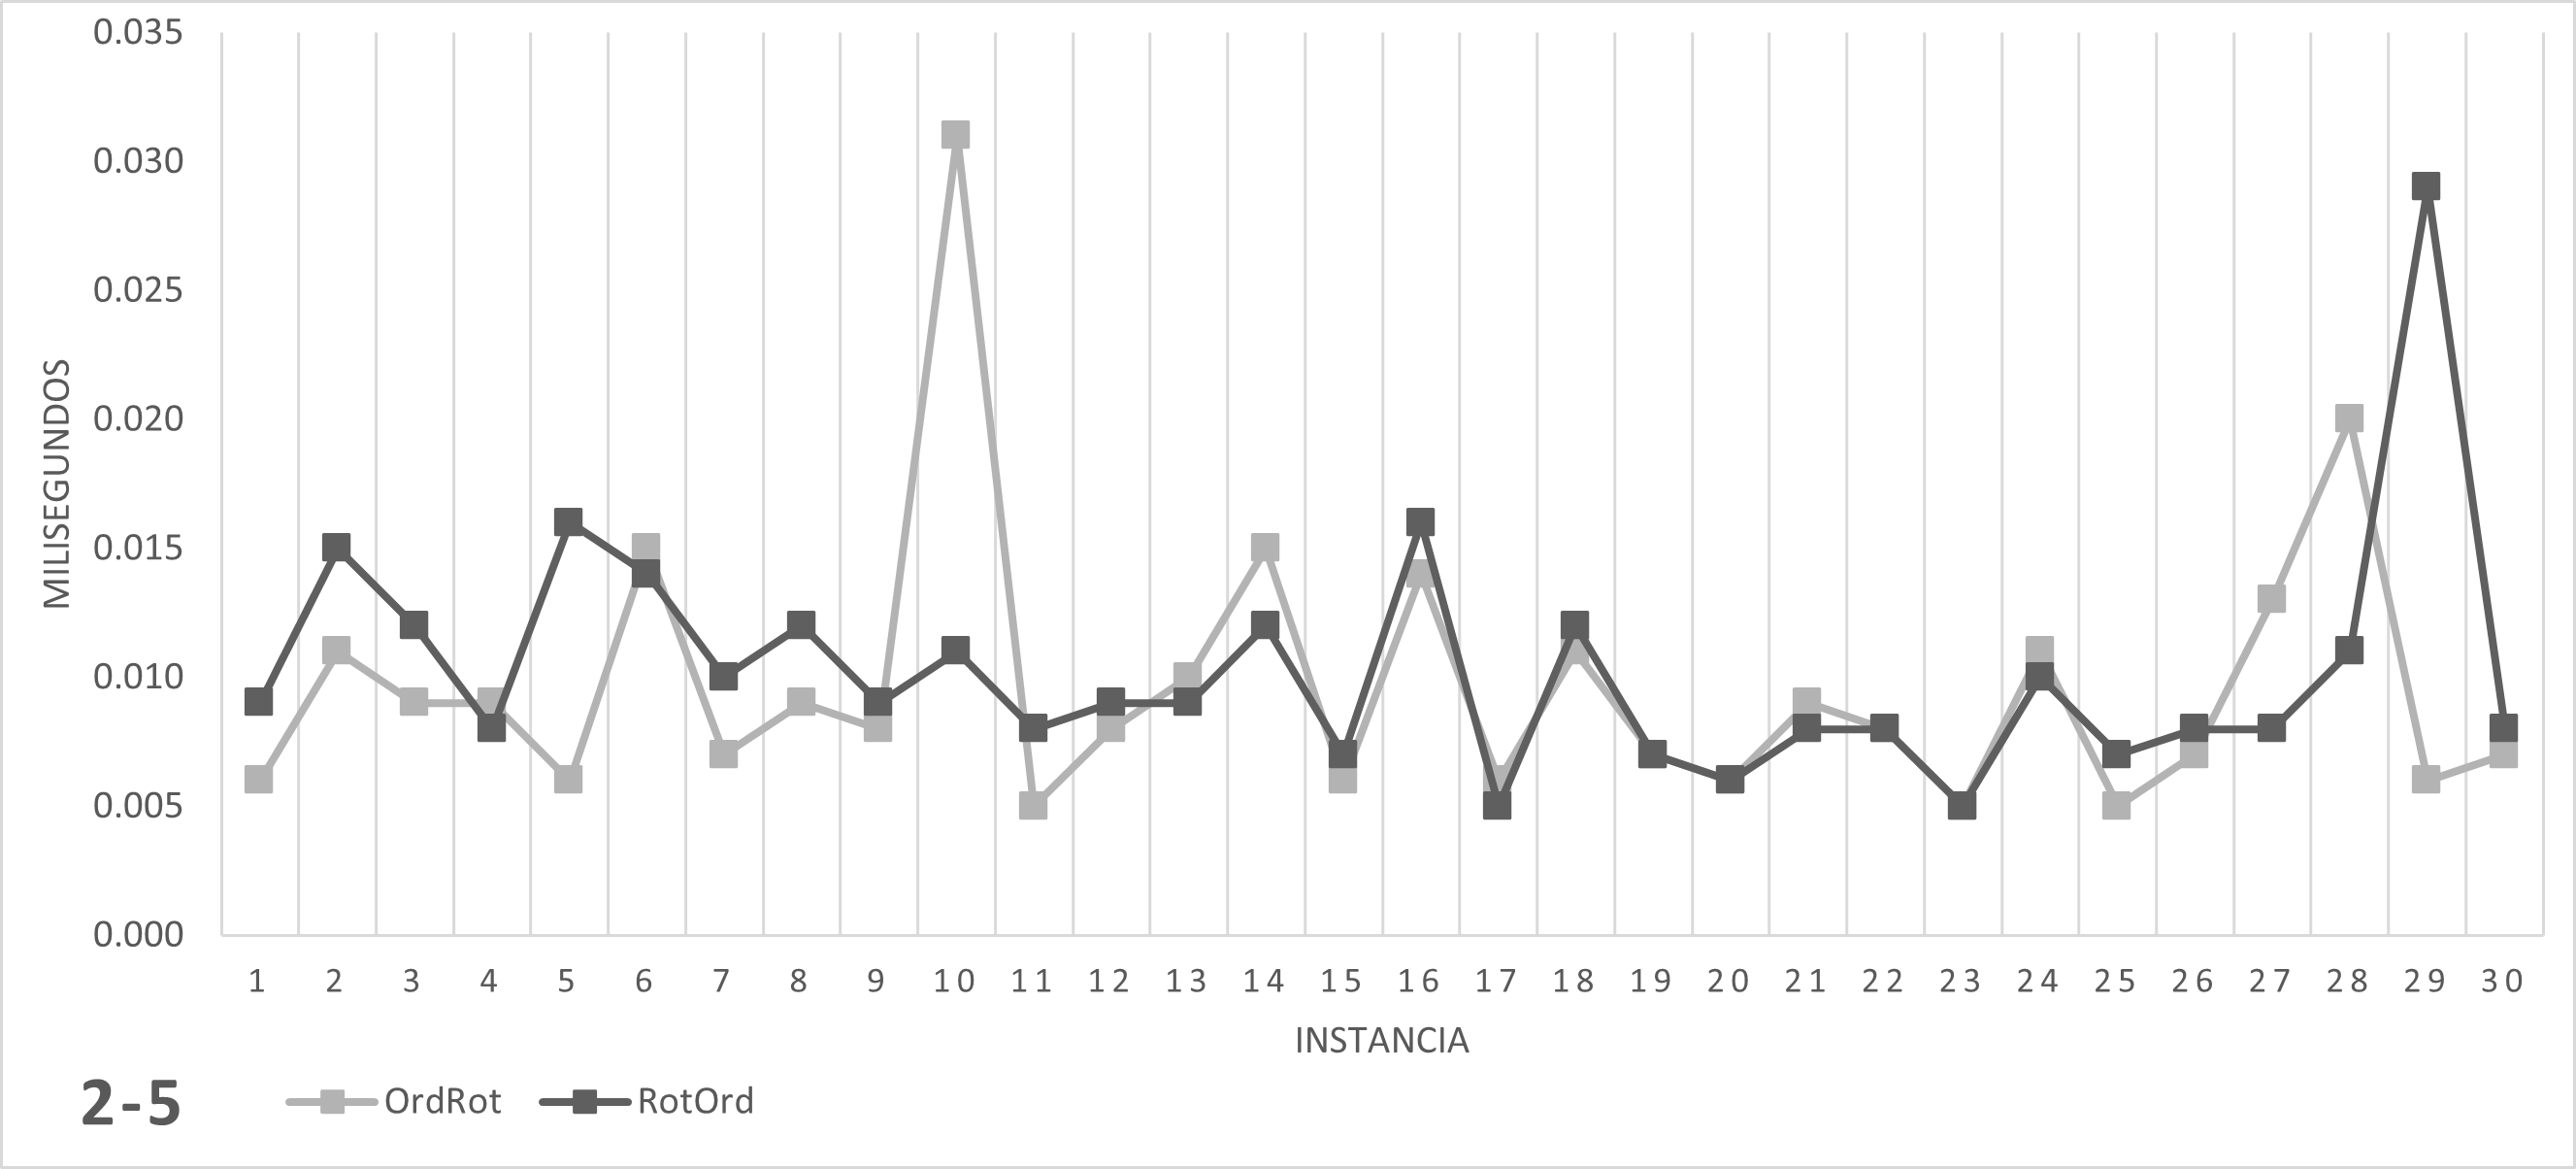
\includegraphics[width=\linewidth]{./img/2-5_t.png}
            \caption*{Tiempo de ejecución.}
            \label{fig:2-5_t}
        \end{minipage}
    \end{adjustwidth}
    \caption{Resultados para instancias de 2-5 bloques.}
    \label{fig:2-5}
\end{figure}

\begin{figure}[H]
    \begin{adjustwidth}{-\marginparwidth}{-\marginparwidth}
        \centering
        \begin{minipage}{.5\linewidth}
            \centering
            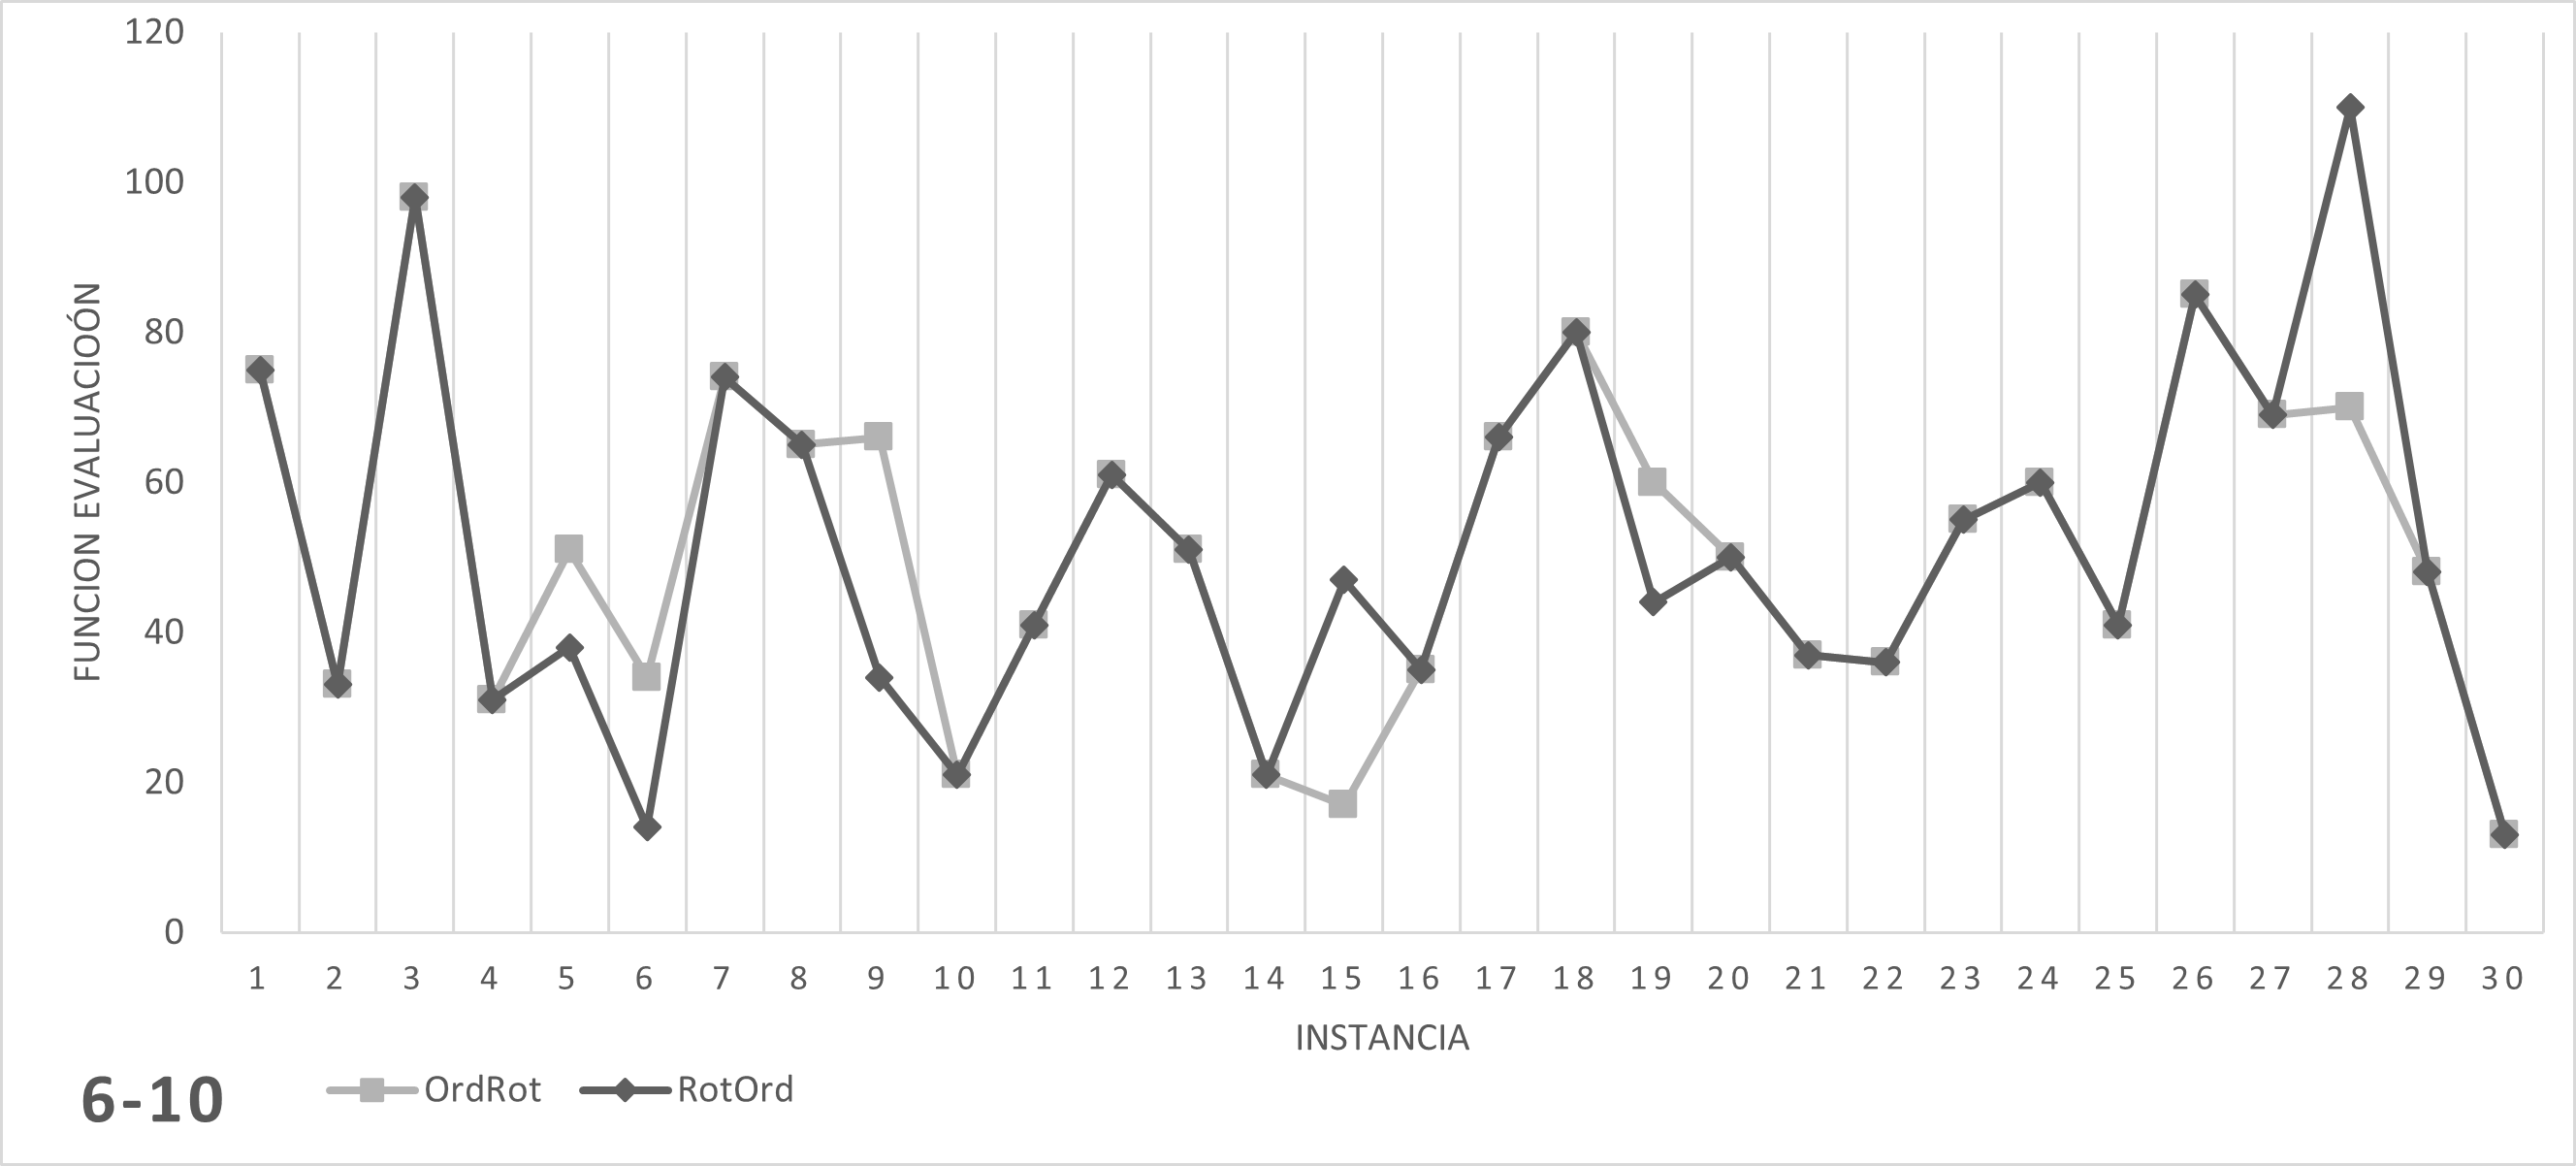
\includegraphics[width=\linewidth]{./img/6-10.png}
            \caption*{Función de evaluación.}
            \label{fig:6-10_g}
        \end{minipage}%
        \begin{minipage}{.5\linewidth}
            \centering
            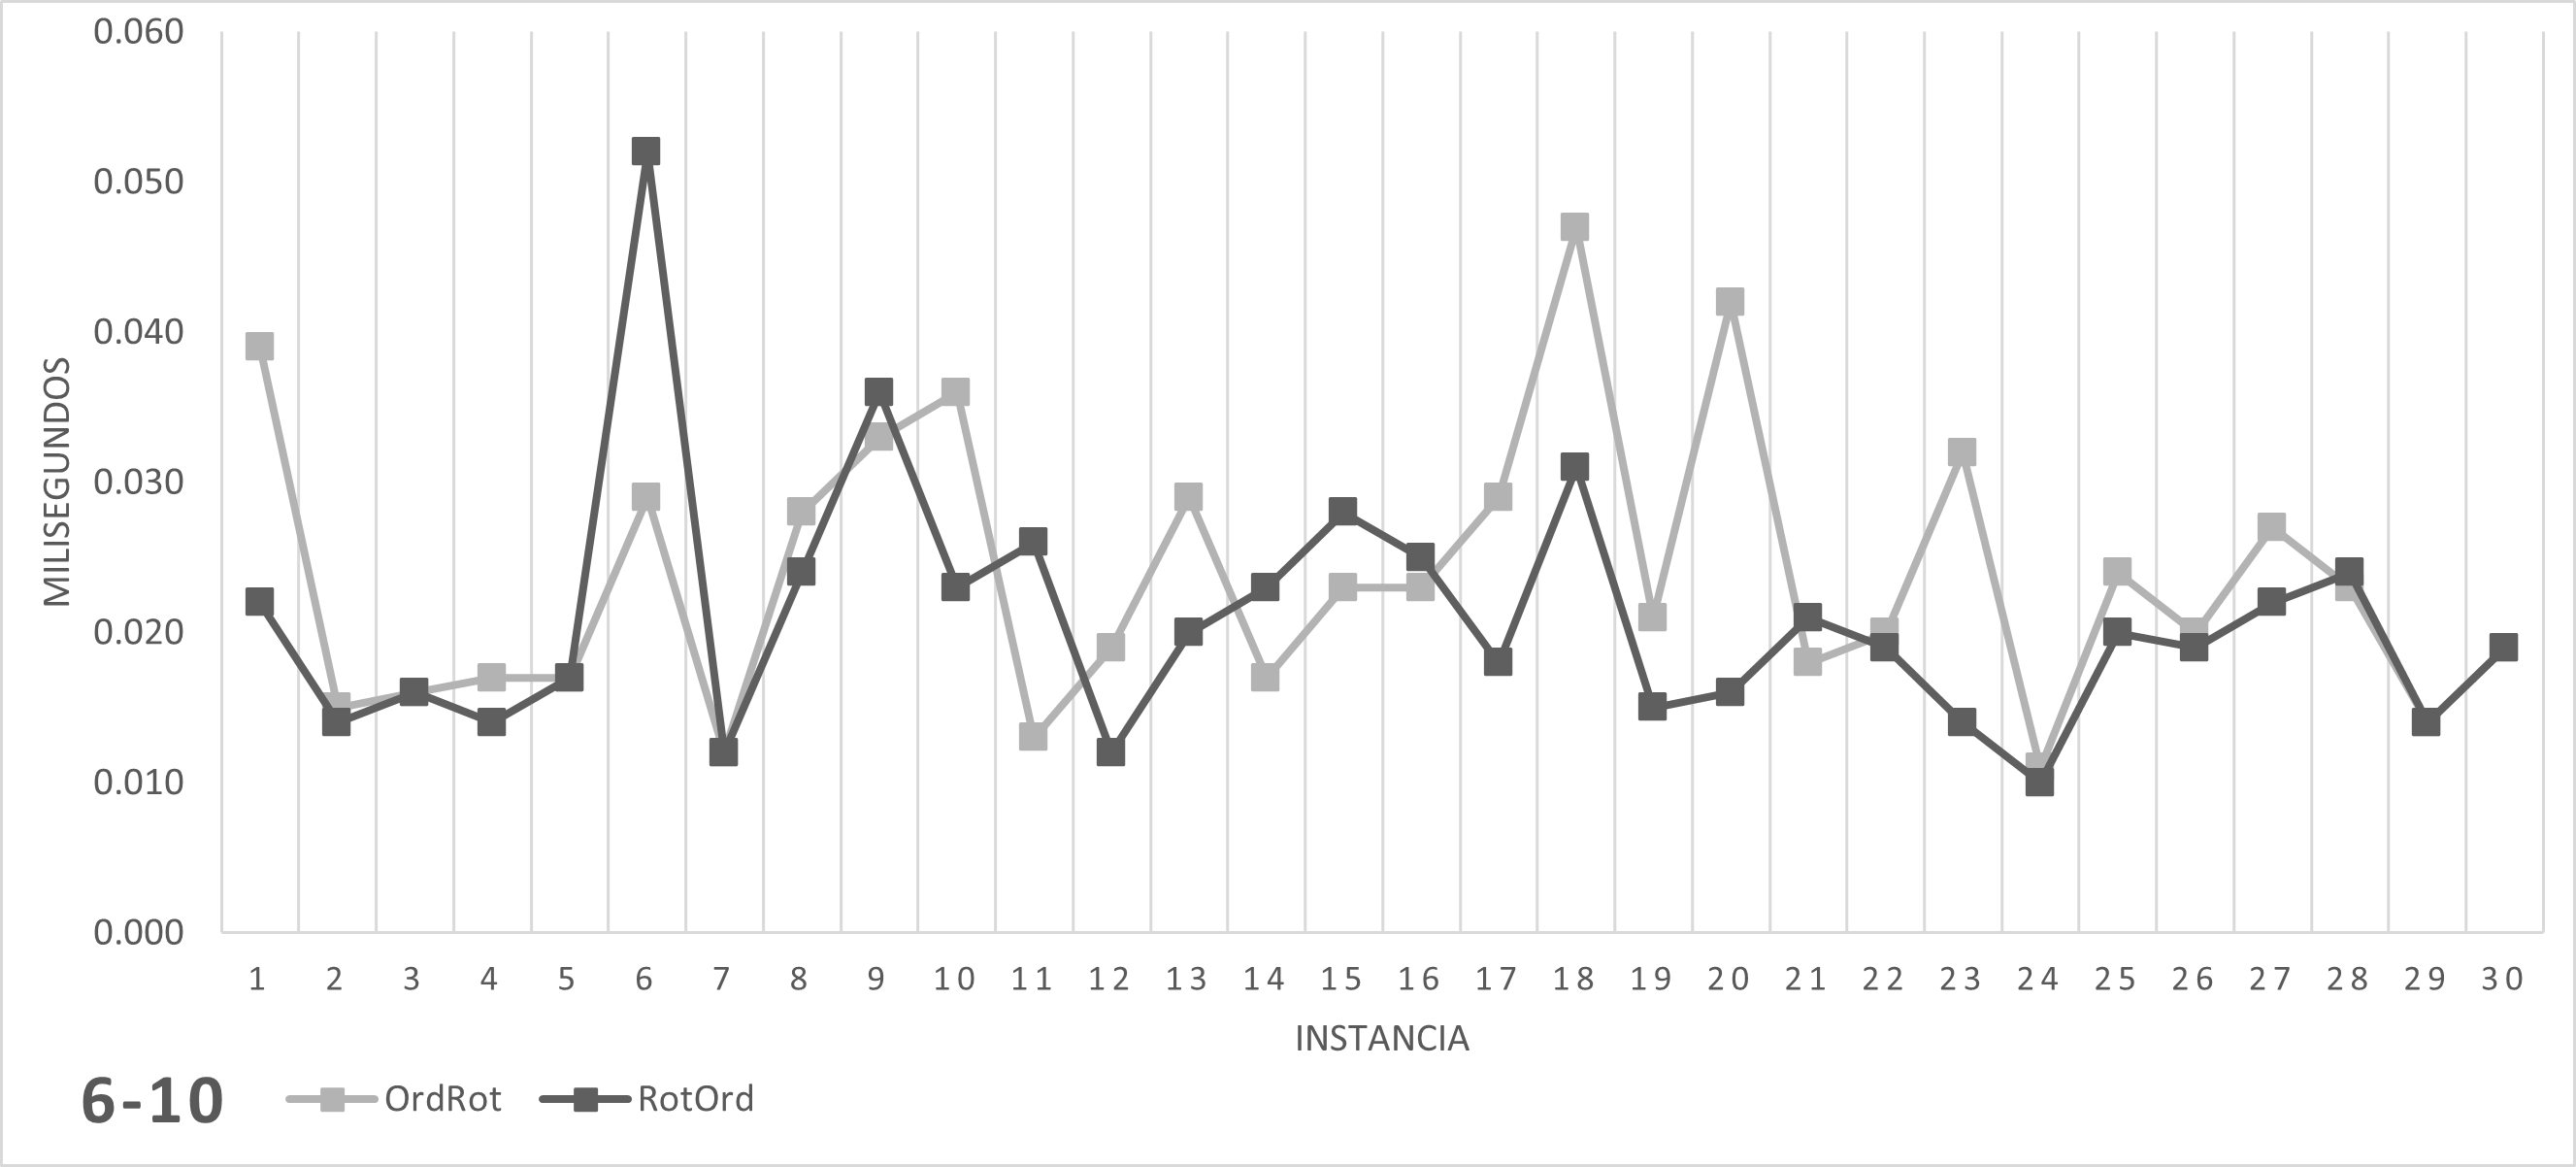
\includegraphics[width=\linewidth]{./img/6-10_t.png}
            \caption*{Tiempo de ejecución.}
            \label{fig:6-10_t}
        \end{minipage}
    \end{adjustwidth}
    \caption{Resultados para instancias de 6-10 bloques.}
    \label{fig:6-10}
\end{figure}

\newpage

\begin{figure}[H]
    \begin{adjustwidth}{-\marginparwidth}{-\marginparwidth}
        \centering
        \begin{minipage}{.5\linewidth}
            \centering
            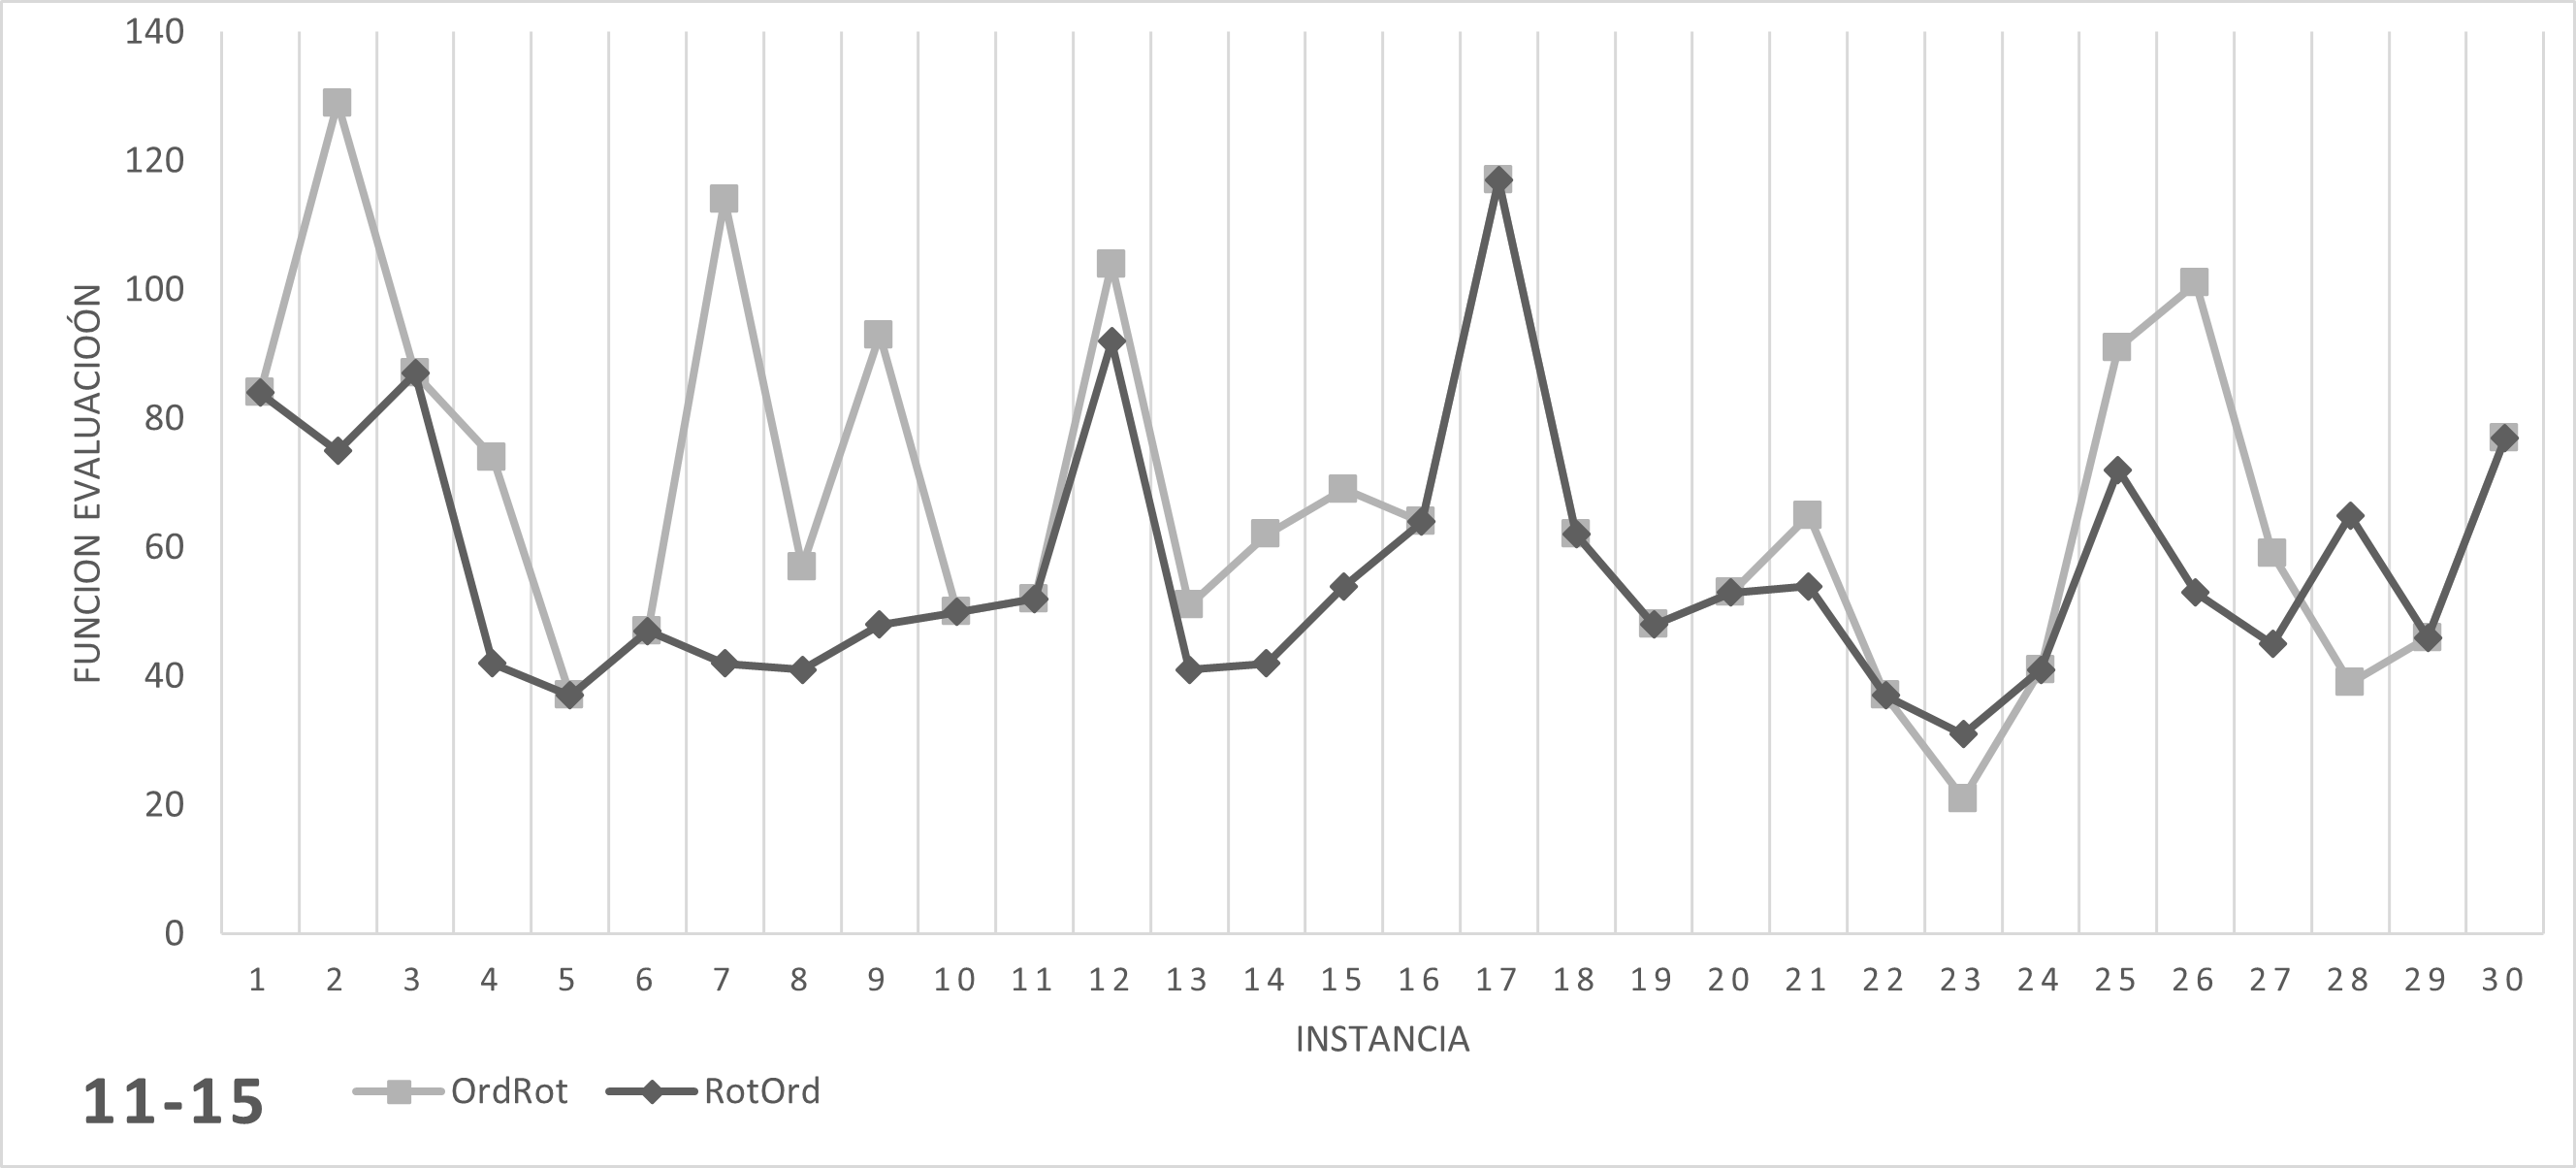
\includegraphics[width=\linewidth]{./img/11-15.png}
            \caption*{Función de evaluación.}
            \label{fig:11-15_g}
        \end{minipage}%
        \begin{minipage}{.5\linewidth}
            \centering
            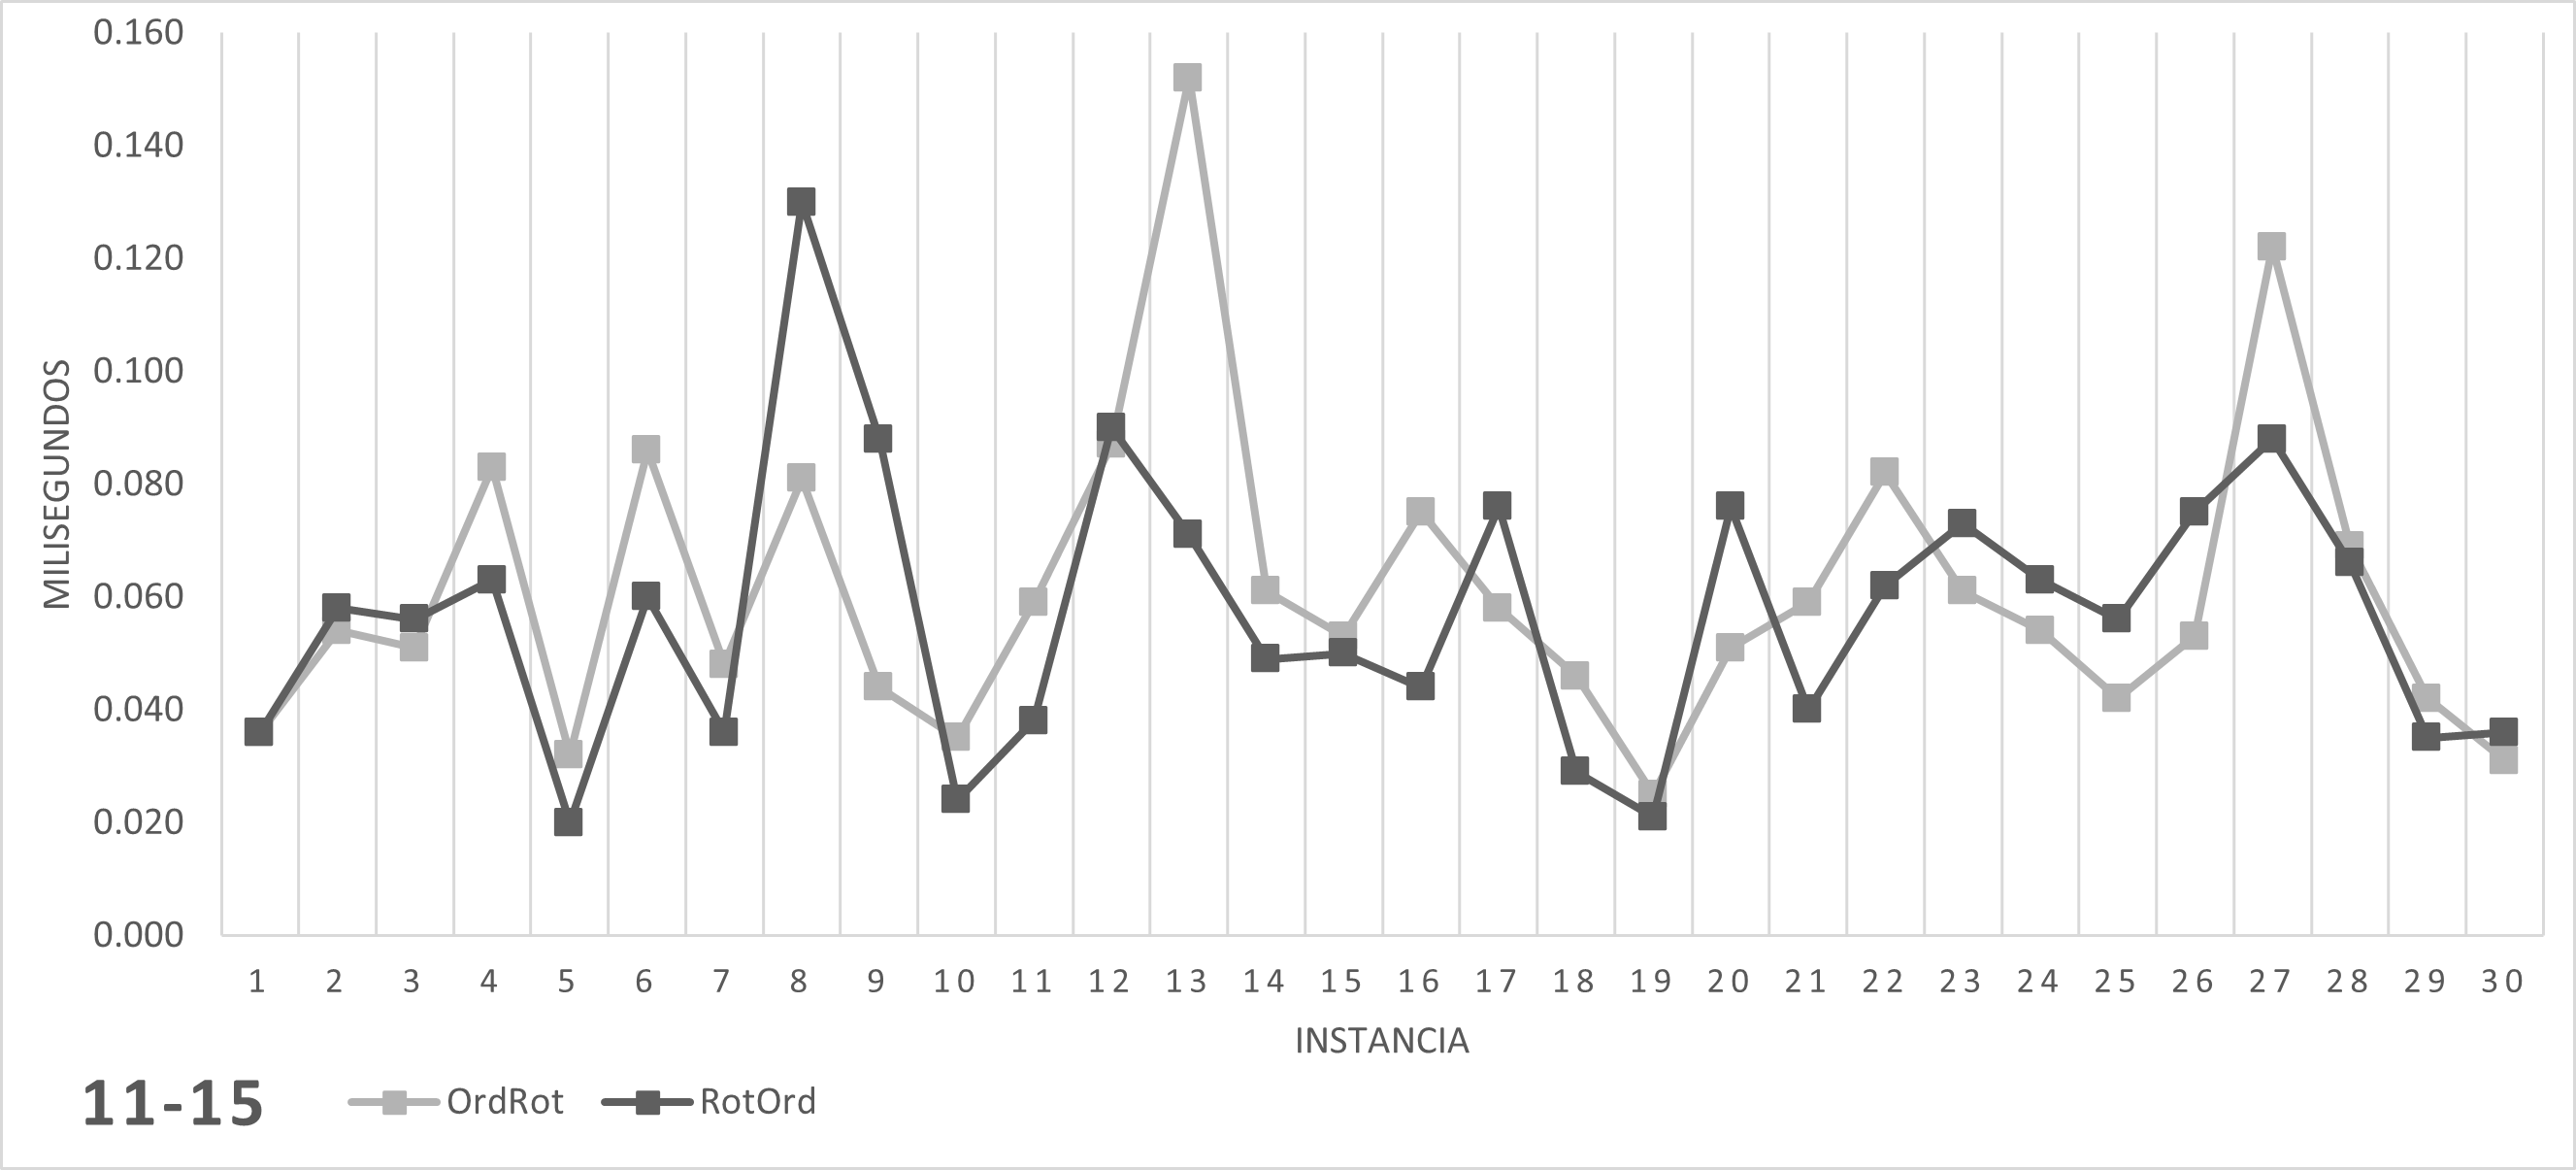
\includegraphics[width=\linewidth]{./img/11-15_t.png}
            \caption*{Tiempo de ejecución.}
            \label{fig:11-15_t}
        \end{minipage}
    \end{adjustwidth}
    \caption{Resultados para instancias de 11-15 bloques.}
    \label{fig:11-15}
\end{figure}

\begin{figure}[H]
    \begin{adjustwidth}{-\marginparwidth}{-\marginparwidth}
        \centering
        \begin{minipage}{.5\linewidth}
            \centering
            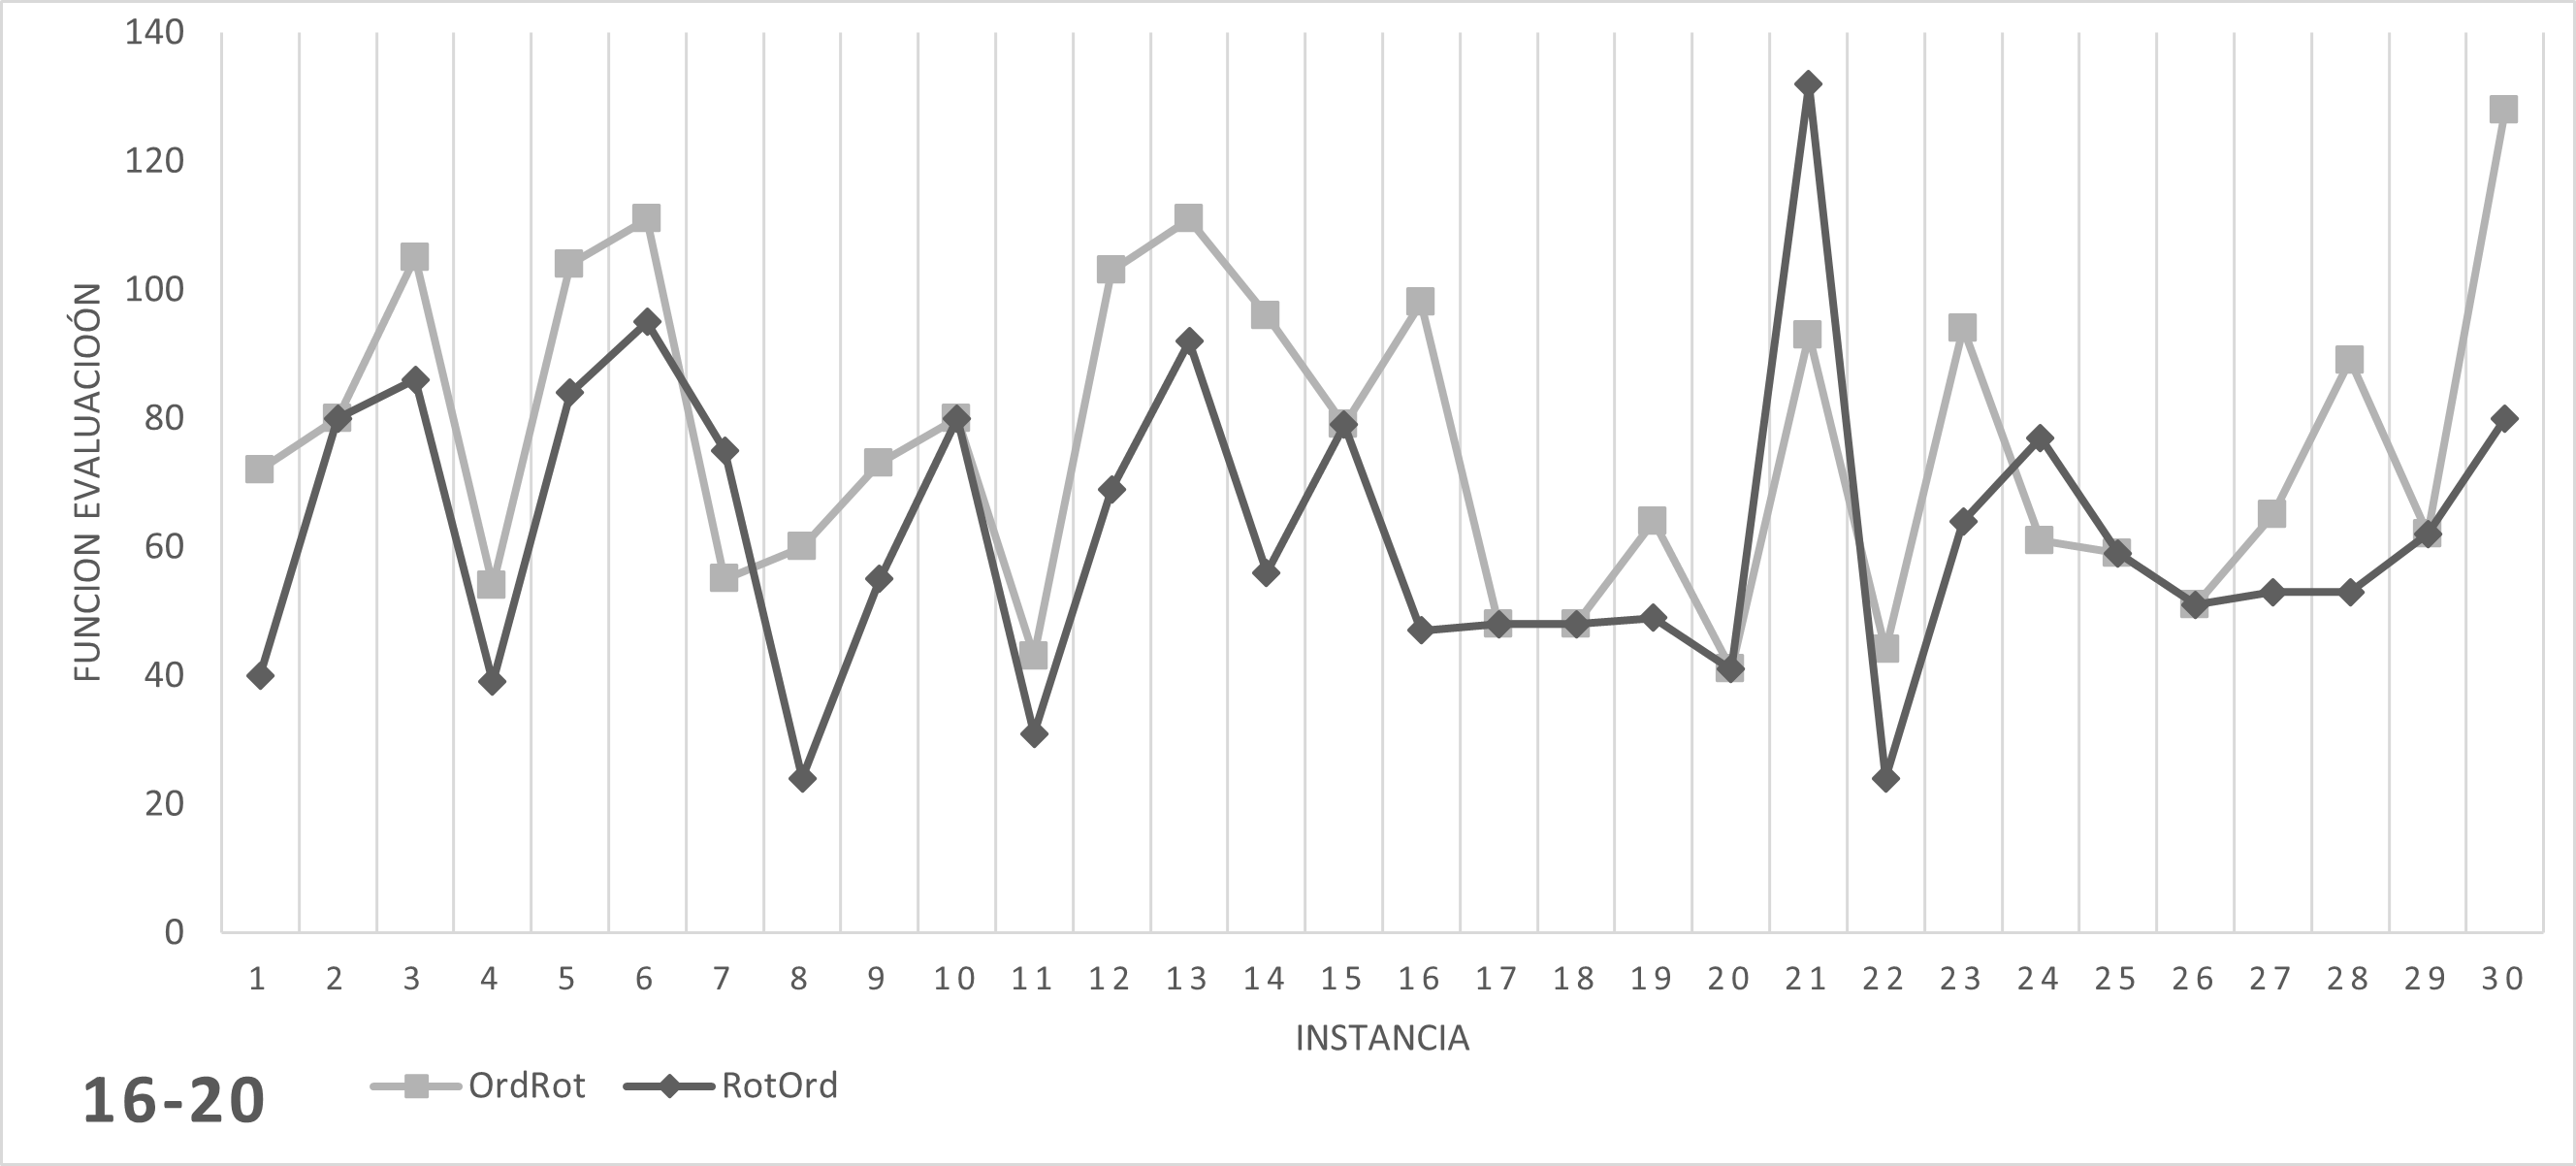
\includegraphics[width=\linewidth]{./img/16-20.png}
            \caption*{Función de evaluación.}
            \label{fig:16-20_g}
        \end{minipage}%
        \begin{minipage}{.5\linewidth}
            \centering
            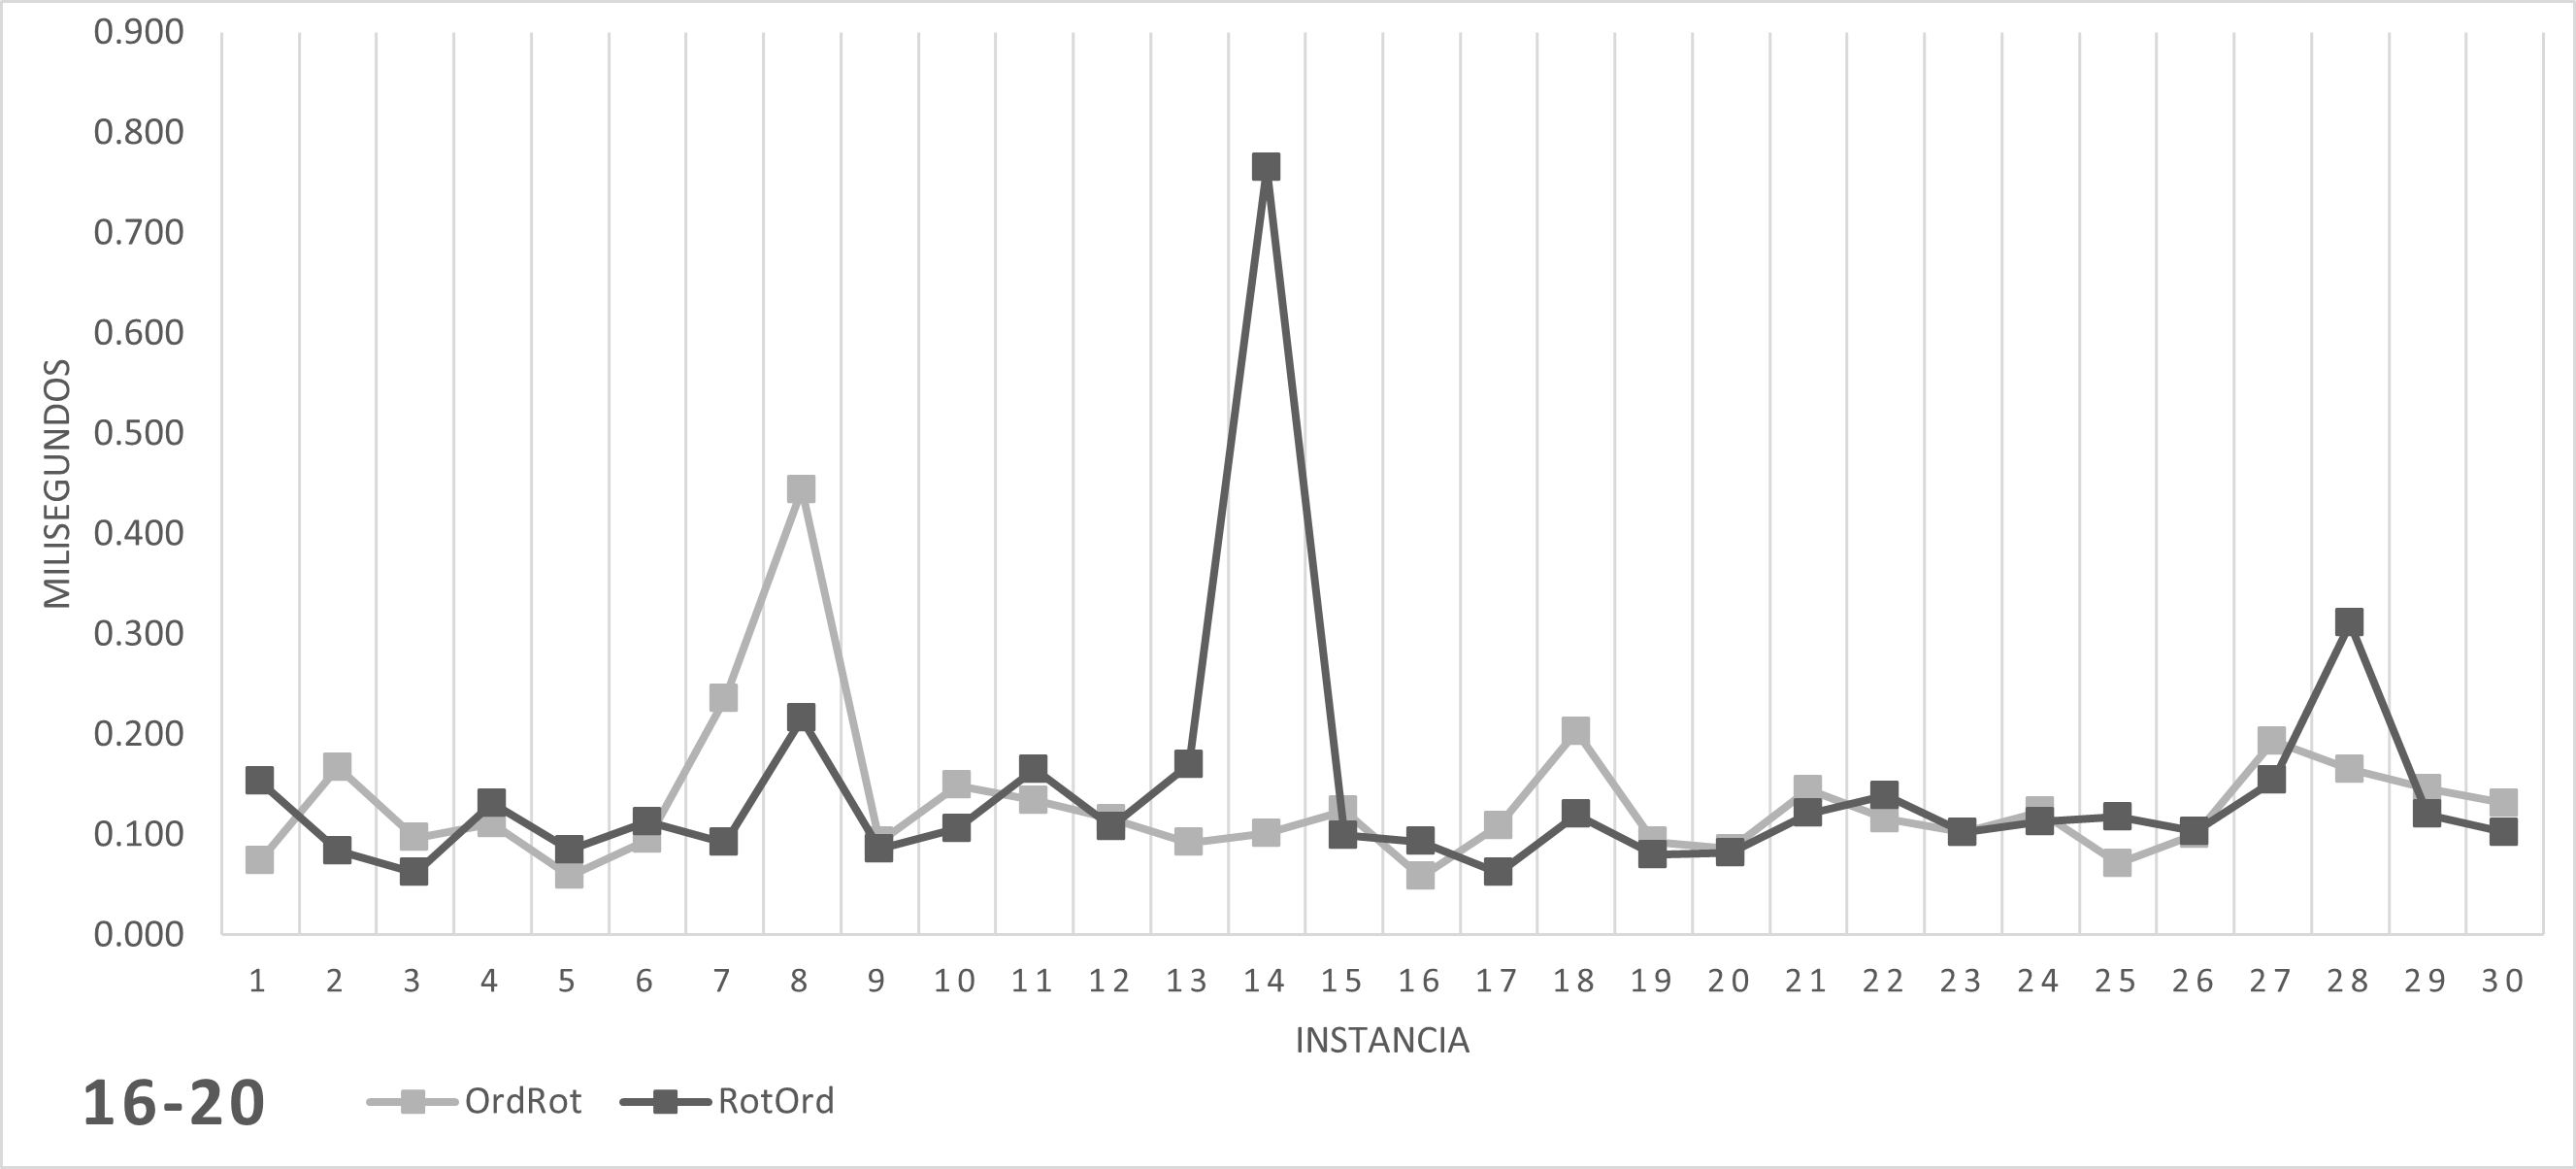
\includegraphics[width=\linewidth]{./img/16-20_t.png}
            \caption*{Tiempo de ejecución.}
            \label{fig:16-20_t}
        \end{minipage}
    \end{adjustwidth}
    \caption{Resultados para instancias de 16-20 bloques.}
    \label{fig:16-20}
\end{figure}







\end{document}
